\documentclass[1p]{elsarticle_modified}
%\bibliographystyle{elsarticle-num}

%\usepackage[colorlinks]{hyperref}
%\usepackage{abbrmath_seonhwa} %\Abb, \Ascr, \Acal ,\Abf, \Afrak
\usepackage{amsfonts}
\usepackage{amssymb}
\usepackage{amsmath}
\usepackage{amsthm}
\usepackage{scalefnt}
\usepackage{amsbsy}
\usepackage{kotex}
\usepackage{caption}
\usepackage{subfig}
\usepackage{color}
\usepackage{graphicx}
\usepackage{xcolor} %% white, black, red, green, blue, cyan, magenta, yellow
\usepackage{float}
\usepackage{setspace}
\usepackage{hyperref}

\usepackage{tikz}
\usetikzlibrary{arrows}

\usepackage{multirow}
\usepackage{array} % fixed length table
\usepackage{hhline}

%%%%%%%%%%%%%%%%%%%%%
\makeatletter
\renewcommand*\env@matrix[1][\arraystretch]{%
	\edef\arraystretch{#1}%
	\hskip -\arraycolsep
	\let\@ifnextchar\new@ifnextchar
	\array{*\c@MaxMatrixCols c}}
\makeatother %https://tex.stackexchange.com/questions/14071/how-can-i-increase-the-line-spacing-in-a-matrix
%%%%%%%%%%%%%%%

\usepackage[normalem]{ulem}

\newcommand{\msout}[1]{\ifmmode\text{\sout{\ensuremath{#1}}}\else\sout{#1}\fi}
%SOURCE: \msout is \stkout macro in https://tex.stackexchange.com/questions/20609/strikeout-in-math-mode

\newcommand{\cancel}[1]{
	\ifmmode
	{\color{red}\msout{#1}}
	\else
	{\color{red}\sout{#1}}
	\fi
}

\newcommand{\add}[1]{
	{\color{blue}\uwave{#1}}
}

\newcommand{\replace}[2]{
	\ifmmode
	{\color{red}\msout{#1}}{\color{blue}\uwave{#2}}
	\else
	{\color{red}\sout{#1}}{\color{blue}\uwave{#2}}
	\fi
}

\newcommand{\Sol}{\mathcal{S}} %segment
\newcommand{\D}{D} %diagram
\newcommand{\A}{\mathcal{A}} %arc


%%%%%%%%%%%%%%%%%%%%%%%%%%%%%5 test

\def\sl{\operatorname{\textup{SL}}(2,\Cbb)}
\def\psl{\operatorname{\textup{PSL}}(2,\Cbb)}
\def\quan{\mkern 1mu \triangleright \mkern 1mu}

\theoremstyle{definition}
\newtheorem{thm}{Theorem}[section]
\newtheorem{prop}[thm]{Proposition}
\newtheorem{lem}[thm]{Lemma}
\newtheorem{ques}[thm]{Question}
\newtheorem{cor}[thm]{Corollary}
\newtheorem{defn}[thm]{Definition}
\newtheorem{exam}[thm]{Example}
\newtheorem{rmk}[thm]{Remark}
\newtheorem{alg}[thm]{Algorithm}

\newcommand{\I}{\sqrt{-1}}
\begin{document}

%\begin{frontmatter}
%
%\title{Boundary parabolic representations of knots up to 8 crossings}
%
%%% Group authors per affiliation:
%\author{Yunhi Cho} 
%\address{Department of Mathematics, University of Seoul, Seoul, Korea}
%\ead{yhcho@uos.ac.kr}
%
%
%\author{Seonhwa Kim} %\fnref{s_kim}}
%\address{Center for Geometry and Physics, Institute for Basic Science, Pohang, 37673, Korea}
%\ead{ryeona17@ibs.re.kr}
%
%\author{Hyuk Kim}
%\address{Department of Mathematical Sciences, Seoul National University, Seoul 08826, Korea}
%\ead{hyukkim@snu.ac.kr}
%
%\author{Seokbeom Yoon}
%\address{Department of Mathematical Sciences, Seoul National University, Seoul, 08826,  Korea}
%\ead{sbyoon15@snu.ac.kr}
%
%\begin{abstract}
%We find all boundary parabolic representation of knots up to 8 crossings.
%
%\end{abstract}
%\begin{keyword}
%    \MSC[2010] 57M25 
%\end{keyword}
%
%\end{frontmatter}

%\linenumbers
%\tableofcontents
%
\newcommand\colored[1]{\textcolor{white}{\rule[-0.35ex]{0.8em}{1.4ex}}\kern-0.8em\color{red} #1}%
%\newcommand\colored[1]{\textcolor{white}{ #1}\kern-2.17ex	\textcolor{white}{ #1}\kern-1.81ex	\textcolor{white}{ #1}\kern-2.15ex\color{red}#1	}

{\Large $\underline{12a_{0656}~(K12a_{0656})}$}

\setlength{\tabcolsep}{10pt}
\renewcommand{\arraystretch}{1.6}
\vspace{1cm}\begin{tabular}{m{100pt}>{\centering\arraybackslash}m{274pt}}
\multirow{5}{120pt}{
	\centering
	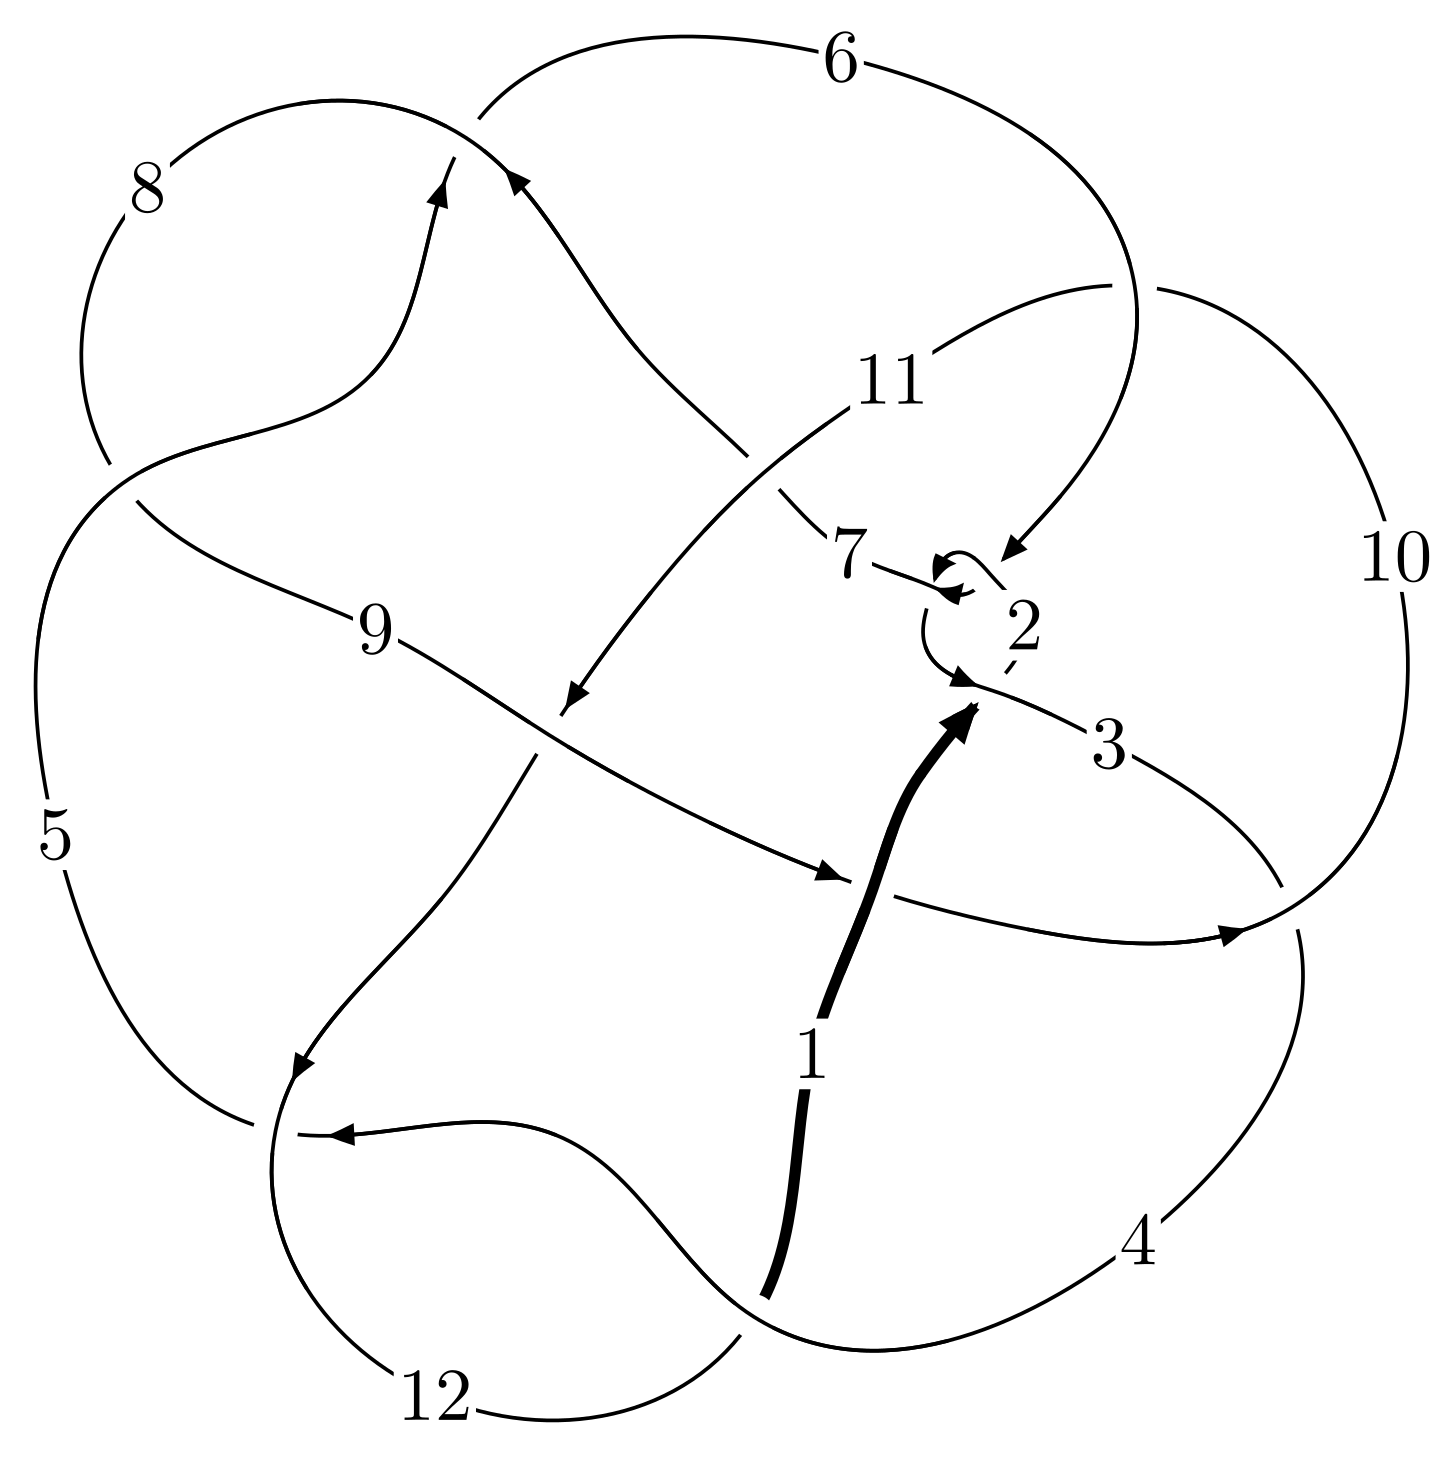
\includegraphics[width=112pt]{../../../GIT/diagram.site/Diagrams/png/1457_12a_0656.png}\\
\ \ \ A knot diagram\footnotemark}&
\allowdisplaybreaks
\textbf{Linearized knot diagam} \\
\cline{2-2}
 &
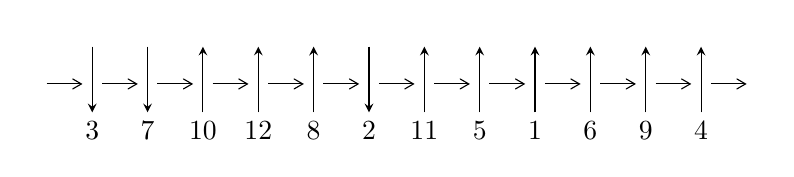
\begin{tikzpicture}[x=20pt, y=17pt]
	% nodes
	\node (C0) at (0, 0) {};
	\node (C1) at (1, 0) {};
	\node (C1U) at (1, +1) {};
	\node (C1D) at (1, -1) {3};

	\node (C2) at (2, 0) {};
	\node (C2U) at (2, +1) {};
	\node (C2D) at (2, -1) {7};

	\node (C3) at (3, 0) {};
	\node (C3U) at (3, +1) {};
	\node (C3D) at (3, -1) {10};

	\node (C4) at (4, 0) {};
	\node (C4U) at (4, +1) {};
	\node (C4D) at (4, -1) {12};

	\node (C5) at (5, 0) {};
	\node (C5U) at (5, +1) {};
	\node (C5D) at (5, -1) {8};

	\node (C6) at (6, 0) {};
	\node (C6U) at (6, +1) {};
	\node (C6D) at (6, -1) {2};

	\node (C7) at (7, 0) {};
	\node (C7U) at (7, +1) {};
	\node (C7D) at (7, -1) {11};

	\node (C8) at (8, 0) {};
	\node (C8U) at (8, +1) {};
	\node (C8D) at (8, -1) {5};

	\node (C9) at (9, 0) {};
	\node (C9U) at (9, +1) {};
	\node (C9D) at (9, -1) {1};

	\node (C10) at (10, 0) {};
	\node (C10U) at (10, +1) {};
	\node (C10D) at (10, -1) {6};

	\node (C11) at (11, 0) {};
	\node (C11U) at (11, +1) {};
	\node (C11D) at (11, -1) {9};

	\node (C12) at (12, 0) {};
	\node (C12U) at (12, +1) {};
	\node (C12D) at (12, -1) {4};
	\node (C13) at (13, 0) {};

	% arrows
	\draw[->,>={angle 60}]
	(C0) edge (C1) (C1) edge (C2) (C2) edge (C3) (C3) edge (C4) (C4) edge (C5) (C5) edge (C6) (C6) edge (C7) (C7) edge (C8) (C8) edge (C9) (C9) edge (C10) (C10) edge (C11) (C11) edge (C12) (C12) edge (C13) ;	\draw[->,>=stealth]
	(C1U) edge (C1D) (C2U) edge (C2D) (C3D) edge (C3U) (C4D) edge (C4U) (C5D) edge (C5U) (C6U) edge (C6D) (C7D) edge (C7U) (C8D) edge (C8U) (C9D) edge (C9U) (C10D) edge (C10U) (C11D) edge (C11U) (C12D) edge (C12U) ;
	\end{tikzpicture} \\
\hhline{~~} \\& 
\textbf{Solving Sequence} \\ \cline{2-2} 
 &
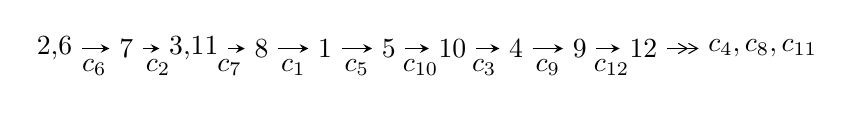
\begin{tikzpicture}[x=23pt, y=7pt]
	% node
	\node (A0) at (-1/8, 0) {2,6};
	\node (A1) at (1, 0) {7};
	\node (A2) at (33/16, 0) {3,11};
	\node (A3) at (25/8, 0) {8};
	\node (A4) at (33/8, 0) {1};
	\node (A5) at (41/8, 0) {5};
	\node (A6) at (49/8, 0) {10};
	\node (A7) at (57/8, 0) {4};
	\node (A8) at (65/8, 0) {9};
	\node (A9) at (73/8, 0) {12};
	\node (C1) at (1/2, -1) {$c_{6}$};
	\node (C2) at (3/2, -1) {$c_{2}$};
	\node (C3) at (21/8, -1) {$c_{7}$};
	\node (C4) at (29/8, -1) {$c_{1}$};
	\node (C5) at (37/8, -1) {$c_{5}$};
	\node (C6) at (45/8, -1) {$c_{10}$};
	\node (C7) at (53/8, -1) {$c_{3}$};
	\node (C8) at (61/8, -1) {$c_{9}$};
	\node (C9) at (69/8, -1) {$c_{12}$};
	\node (A10) at (11, 0) {$c_{4},c_{8},c_{11}$};

	% edge
	\draw[->,>=stealth]	
	(A0) edge (A1) (A1) edge (A2) (A2) edge (A3) (A3) edge (A4) (A4) edge (A5) (A5) edge (A6) (A6) edge (A7) (A7) edge (A8) (A8) edge (A9) ;
	\draw[->>,>={angle 60}]	
	(A9) edge (A10);
\end{tikzpicture} \\ 

\end{tabular} \\

\footnotetext{
The image of knot diagram is generated by the software ``\textbf{Draw programme}" developed by Andrew Bartholomew(\url{http://www.layer8.co.uk/maths/draw/index.htm\#Running-draw}), where we modified some parts for our purpose(\url{https://github.com/CATsTAILs/LinksPainter}).
}\phantom \\ \newline 
\centering \textbf{Ideals for irreducible components\footnotemark of $X_{\text{par}}$} 
 
\begin{align*}
I^u_{1}&=\langle 
-9540655 u^{40}-39881332 u^{39}+\cdots+2811062 b+78036718,\\
\phantom{I^u_{1}}&\phantom{= \langle  }177709945 u^{40}+1366370774 u^{39}+\cdots+16866372 a+2496378600,\;u^{41}+8 u^{40}+\cdots+102 u+12\rangle \\
I^u_{2}&=\langle 
3.46819\times10^{21} a u^{52}-3.39067\times10^{24} u^{52}+\cdots-1.10739\times10^{22} a+2.55339\times10^{24},\\
\phantom{I^u_{2}}&\phantom{= \langle  }-2.28935\times10^{21} a u^{52}+1.20458\times10^{21} u^{52}+\cdots+3.67777\times10^{21} a-1.92411\times10^{20},\\
\phantom{I^u_{2}}&\phantom{= \langle  }u^{53}-3 u^{52}+\cdots-7 u+3\rangle \\
I^u_{3}&=\langle 
-2 u^{15}-2 u^{14}+\cdots+b+1,\\
\phantom{I^u_{3}}&\phantom{= \langle  }2 u^{15}+5 u^{14}-12 u^{12}-10 u^{11}+11 u^{10}+21 u^9-2 u^8-26 u^7-9 u^6+19 u^5+11 u^4-5 u^3-2 u^2+a+3 u,\\
\phantom{I^u_{3}}&\phantom{= \langle  }u^{16}+3 u^{15}+2 u^{14}-5 u^{13}-9 u^{12}+13 u^{10}+8 u^9-11 u^8-15 u^7+3 u^6+13 u^5+4 u^4-4 u^3- u^2+2 u+1\rangle \\
I^u_{4}&=\langle 
- u^6 a+3 u^5 a-9 u^6+2 u^4 a+6 u^5-5 u^3 a+11 u^4-6 u^2 a-3 u^3+6 a u-19 u^2+7 b+3 a-2 u+6,\\
\phantom{I^u_{4}}&\phantom{= \langle  }- u^6 a+2 u^4 a-3 u^5+2 u^4-3 u^2 a+2 u^3+a^2-2 a u+2 a-5 u+1,\;u^7- u^6- u^5+u^4+2 u^3- u^2- u+1\rangle \\
\\
\end{align*}
\raggedright * 4 irreducible components of $\dim_{\mathbb{C}}=0$, with total 177 representations.\\
\footnotetext{All coefficients of polynomials are rational numbers. But the coefficients are sometimes approximated in decimal forms when there is not enough margin.}
\newpage
\renewcommand{\arraystretch}{1}
\centering \section*{I. $I^u_{1}= \langle -9.54\times10^{6} u^{40}-3.99\times10^{7} u^{39}+\cdots+2.81\times10^{6} b+7.80\times10^{7},\;1.78\times10^{8} u^{40}+1.37\times10^{9} u^{39}+\cdots+1.69\times10^{7} a+2.50\times10^{9},\;u^{41}+8 u^{40}+\cdots+102 u+12 \rangle$}
\flushleft \textbf{(i) Arc colorings}\\
\begin{tabular}{m{7pt} m{180pt} m{7pt} m{180pt} }
\flushright $a_{2}=$&$\begin{pmatrix}0\\u\end{pmatrix}$ \\
\flushright $a_{6}=$&$\begin{pmatrix}1\\0\end{pmatrix}$ \\
\flushright $a_{7}=$&$\begin{pmatrix}1\\u^2\end{pmatrix}$ \\
\flushright $a_{3}=$&$\begin{pmatrix}- u\\- u^3+u\end{pmatrix}$ \\
\flushright $a_{11}=$&$\begin{pmatrix}-10.5363 u^{40}-81.0115 u^{39}+\cdots-1142.34 u-148.009\\3.39397 u^{40}+14.1873 u^{39}+\cdots-189.050 u-27.7606\end{pmatrix}$ \\
\flushright $a_{8}=$&$\begin{pmatrix}11.9344 u^{40}+81.1701 u^{39}+\cdots+642.098 u+78.2302\\5.42199 u^{40}+44.9429 u^{39}+\cdots+841.464 u+112.318\end{pmatrix}$ \\
\flushright $a_{1}=$&$\begin{pmatrix}u^3\\u^5- u^3+u\end{pmatrix}$ \\
\flushright $a_{5}=$&$\begin{pmatrix}2.23943 u^{40}+11.2000 u^{39}+\cdots-81.5979 u-12.3360\\7.54178 u^{40}+56.4150 u^{39}+\cdots+626.918 u+78.4362\end{pmatrix}$ \\
\flushright $a_{10}=$&$\begin{pmatrix}-13.9303 u^{40}-95.1988 u^{39}+\cdots-953.293 u-120.249\\3.39397 u^{40}+14.1873 u^{39}+\cdots-189.050 u-27.7606\end{pmatrix}$ \\
\flushright $a_{4}=$&$\begin{pmatrix}8.93120 u^{40}+49.3410 u^{39}+\cdots-43.6295 u-16.1139\\10.7792 u^{40}+85.8051 u^{39}+\cdots+1221.80 u+158.128\end{pmatrix}$ \\
\flushright $a_{9}=$&$\begin{pmatrix}8.17922 u^{40}+62.6496 u^{39}+\cdots+848.799 u+110.731\\1.12373 u^{40}+13.0388 u^{39}+\cdots+341.462 u+45.5333\end{pmatrix}$ \\
\flushright $a_{12}=$&$\begin{pmatrix}-16.6903 u^{40}-127.083 u^{39}+\cdots-1863.89 u-244.521\\8.31913 u^{40}+52.5805 u^{39}+\cdots+336.750 u+39.1452\end{pmatrix}$\\&\end{tabular}
\flushleft \textbf{(ii) Obstruction class $= -1$}\\~\\
\flushleft \textbf{(iii) Cusp Shapes $= \frac{50634926}{1405531} u^{40}+\frac{355341377}{1405531} u^{39}+\cdots+\frac{2555447816}{1405531} u+\frac{305571258}{1405531}$}\\~\\
\newpage\renewcommand{\arraystretch}{1}
\flushleft \textbf{(iv) u-Polynomials at the component}\newline \\
\begin{tabular}{m{50pt}|m{274pt}}
Crossings & \hspace{64pt}u-Polynomials at each crossing \\
\hline $$\begin{aligned}c_{1}\end{aligned}$$&$\begin{aligned}
&u^{41}+14 u^{40}+\cdots+1308 u+144
\end{aligned}$\\
\hline $$\begin{aligned}c_{2},c_{6}\end{aligned}$$&$\begin{aligned}
&u^{41}-8 u^{40}+\cdots+102 u-12
\end{aligned}$\\
\hline $$\begin{aligned}c_{3},c_{10}\end{aligned}$$&$\begin{aligned}
&u^{41}+12 u^{39}+\cdots+13 u-7
\end{aligned}$\\
\hline $$\begin{aligned}c_{4},c_{5},c_{8}\\c_{12}\end{aligned}$$&$\begin{aligned}
&u^{41}+u^{40}+\cdots+5 u-1
\end{aligned}$\\
\hline $$\begin{aligned}c_{7},c_{9}\end{aligned}$$&$\begin{aligned}
&u^{41}+3 u^{40}+\cdots-10 u-1
\end{aligned}$\\
\hline $$\begin{aligned}c_{11}\end{aligned}$$&$\begin{aligned}
&u^{41}+29 u^{40}+\cdots-31212 u-2196
\end{aligned}$\\
\hline
\end{tabular}\\~\\
\newpage\renewcommand{\arraystretch}{1}
\flushleft \textbf{(v) Riley Polynomials at the component}\newline \\
\begin{tabular}{m{50pt}|m{274pt}}
Crossings & \hspace{64pt}Riley Polynomials at each crossing \\
\hline $$\begin{aligned}c_{1}\end{aligned}$$&$\begin{aligned}
&y^{41}+18 y^{40}+\cdots+259056 y-20736
\end{aligned}$\\
\hline $$\begin{aligned}c_{2},c_{6}\end{aligned}$$&$\begin{aligned}
&y^{41}-14 y^{40}+\cdots+1308 y-144
\end{aligned}$\\
\hline $$\begin{aligned}c_{3},c_{10}\end{aligned}$$&$\begin{aligned}
&y^{41}+24 y^{40}+\cdots-2197 y-49
\end{aligned}$\\
\hline $$\begin{aligned}c_{4},c_{5},c_{8}\\c_{12}\end{aligned}$$&$\begin{aligned}
&y^{41}+41 y^{40}+\cdots+13 y-1
\end{aligned}$\\
\hline $$\begin{aligned}c_{7},c_{9}\end{aligned}$$&$\begin{aligned}
&y^{41}-3 y^{40}+\cdots-44 y-1
\end{aligned}$\\
\hline $$\begin{aligned}c_{11}\end{aligned}$$&$\begin{aligned}
&y^{41}- y^{40}+\cdots+18265752 y-4822416
\end{aligned}$\\
\hline
\end{tabular}\\~\\
\newpage\flushleft \textbf{(vi) Complex Volumes and Cusp Shapes}
$$\begin{array}{c|c|c}  
\text{Solutions to }I^u_{1}& \I (\text{vol} + \sqrt{-1}CS) & \text{Cusp shape}\\
 \hline 
\begin{aligned}
u &= \phantom{-}0.885459 + 0.468568 I \\
a &= \phantom{-}0.74140 + 2.12496 I \\
b &= \phantom{-}0.14627 + 1.57300 I\end{aligned}
 & -8.61867 - 1.89974 I & -0.41209 + 3.72876 I \\ \hline\begin{aligned}
u &= \phantom{-}0.885459 - 0.468568 I \\
a &= \phantom{-}0.74140 - 2.12496 I \\
b &= \phantom{-}0.14627 - 1.57300 I\end{aligned}
 & -8.61867 + 1.89974 I & -0.41209 - 3.72876 I \\ \hline\begin{aligned}
u &= -0.638864 + 0.751208 I \\
a &= \phantom{-}0.138021 + 0.619122 I \\
b &= \phantom{-}1.31734 - 1.20105 I\end{aligned}
 & -4.97109 - 2.38814 I & \phantom{-}1.29196 + 2.16768 I \\ \hline\begin{aligned}
u &= -0.638864 - 0.751208 I \\
a &= \phantom{-}0.138021 - 0.619122 I \\
b &= \phantom{-}1.31734 + 1.20105 I\end{aligned}
 & -4.97109 + 2.38814 I & \phantom{-}1.29196 - 2.16768 I \\ \hline\begin{aligned}
u &= \phantom{-}1.023760 + 0.040551 I \\
a &= -0.89941 + 2.43314 I \\
b &= -0.63878 + 1.63015 I\end{aligned}
 & -10.53450 - 2.01458 I & -6.45706 + 3.63025 I \\ \hline\begin{aligned}
u &= \phantom{-}1.023760 - 0.040551 I \\
a &= -0.89941 - 2.43314 I \\
b &= -0.63878 - 1.63015 I\end{aligned}
 & -10.53450 + 2.01458 I & -6.45706 - 3.63025 I \\ \hline\begin{aligned}
u &= -0.336434 + 0.998716 I \\
a &= -0.244879 - 0.078110 I \\
b &= -0.428361 - 0.703700 I\end{aligned}
 & -5.98718 + 8.31828 I & \phantom{-}0.77031 - 8.90553 I \\ \hline\begin{aligned}
u &= -0.336434 - 0.998716 I \\
a &= -0.244879 + 0.078110 I \\
b &= -0.428361 + 0.703700 I\end{aligned}
 & -5.98718 - 8.31828 I & \phantom{-}0.77031 + 8.90553 I \\ \hline\begin{aligned}
u &= \phantom{-}0.852689 + 0.638581 I \\
a &= -0.665891 - 1.232780 I \\
b &= -0.201595 - 1.034500 I\end{aligned}
 & \phantom{-}3.45937 - 2.49348 I & \phantom{-}17.3496 + 3.7147 I \\ \hline\begin{aligned}
u &= \phantom{-}0.852689 - 0.638581 I \\
a &= -0.665891 + 1.232780 I \\
b &= -0.201595 + 1.034500 I\end{aligned}
 & \phantom{-}3.45937 + 2.49348 I & \phantom{-}17.3496 - 3.7147 I\\
 \hline 
 \end{array}$$\newpage$$\begin{array}{c|c|c}  
\text{Solutions to }I^u_{1}& \I (\text{vol} + \sqrt{-1}CS) & \text{Cusp shape}\\
 \hline 
\begin{aligned}
u &= -0.984331 + 0.435389 I \\
a &= -1.49599 + 0.52826 I \\
b &= \phantom{-}0.247555 + 0.788723 I\end{aligned}
 & -8.39285 + 3.15435 I & -2.00509 - 3.79246 I \\ \hline\begin{aligned}
u &= -0.984331 - 0.435389 I \\
a &= -1.49599 - 0.52826 I \\
b &= \phantom{-}0.247555 - 0.788723 I\end{aligned}
 & -8.39285 - 3.15435 I & -2.00509 + 3.79246 I \\ \hline\begin{aligned}
u &= -0.558695 + 0.934797 I \\
a &= -0.224063 + 0.056775 I \\
b &= -1.00584 + 1.24085 I\end{aligned}
 & -4.7480 - 13.5144 I & \phantom{-}3.83057 + 6.47722 I \\ \hline\begin{aligned}
u &= -0.558695 - 0.934797 I \\
a &= -0.224063 - 0.056775 I \\
b &= -1.00584 - 1.24085 I\end{aligned}
 & -4.7480 + 13.5144 I & \phantom{-}3.83057 - 6.47722 I \\ \hline\begin{aligned}
u &= -0.578439 + 0.934242 I \\
a &= \phantom{-}0.180422 + 0.011630 I \\
b &= \phantom{-}0.828821 - 0.703301 I\end{aligned}
 & \phantom{-}4.82087 - 2.96510 I & \phantom{-}11.89661 + 4.32984 I \\ \hline\begin{aligned}
u &= -0.578439 - 0.934242 I \\
a &= \phantom{-}0.180422 - 0.011630 I \\
b &= \phantom{-}0.828821 + 0.703301 I\end{aligned}
 & \phantom{-}4.82087 + 2.96510 I & \phantom{-}11.89661 - 4.32984 I \\ \hline\begin{aligned}
u &= \phantom{-}0.911339 + 0.643598 I \\
a &= \phantom{-}0.442568 + 0.534189 I \\
b &= \phantom{-}0.213097 + 0.483788 I\end{aligned}
 & -1.08260 - 2.39919 I & \phantom{-}2.82500 + 2.36815 I \\ \hline\begin{aligned}
u &= \phantom{-}0.911339 - 0.643598 I \\
a &= \phantom{-}0.442568 - 0.534189 I \\
b &= \phantom{-}0.213097 - 0.483788 I\end{aligned}
 & -1.08260 + 2.39919 I & \phantom{-}2.82500 - 2.36815 I \\ \hline\begin{aligned}
u &= \phantom{-}0.450241 + 1.042540 I \\
a &= \phantom{-}0.082525 + 0.244030 I \\
b &= -0.042347 + 0.250005 I\end{aligned}
 & \phantom{-}0.63600 - 2.52874 I & \phantom{-}18.1134 + 18.3545 I \\ \hline\begin{aligned}
u &= \phantom{-}0.450241 - 1.042540 I \\
a &= \phantom{-}0.082525 - 0.244030 I \\
b &= -0.042347 - 0.250005 I\end{aligned}
 & \phantom{-}0.63600 + 2.52874 I & \phantom{-}18.1134 - 18.3545 I\\
 \hline 
 \end{array}$$\newpage$$\begin{array}{c|c|c}  
\text{Solutions to }I^u_{1}& \I (\text{vol} + \sqrt{-1}CS) & \text{Cusp shape}\\
 \hline 
\begin{aligned}
u &= -0.905940 + 0.723310 I \\
a &= -1.206950 + 0.270424 I \\
b &= \phantom{-}0.06050 + 1.48050 I\end{aligned}
 & -6.88574 + 2.77950 I & -2.52803 - 2.69400 I \\ \hline\begin{aligned}
u &= -0.905940 - 0.723310 I \\
a &= -1.206950 - 0.270424 I \\
b &= \phantom{-}0.06050 - 1.48050 I\end{aligned}
 & -6.88574 - 2.77950 I & -2.52803 + 2.69400 I \\ \hline\begin{aligned}
u &= \phantom{-}1.156170 + 0.163202 I \\
a &= \phantom{-}0.054861 + 1.154130 I \\
b &= -0.011284 + 0.831483 I\end{aligned}
 & -2.60053 - 1.63849 I & \phantom{-}1.29829 + 3.72995 I \\ \hline\begin{aligned}
u &= \phantom{-}1.156170 - 0.163202 I \\
a &= \phantom{-}0.054861 - 1.154130 I \\
b &= -0.011284 - 0.831483 I\end{aligned}
 & -2.60053 + 1.63849 I & \phantom{-}1.29829 - 3.72995 I \\ \hline\begin{aligned}
u &= -1.017490 + 0.598781 I \\
a &= -0.48971 + 1.36588 I \\
b &= \phantom{-}0.938580 + 0.636689 I\end{aligned}
 & \phantom{-}0.01859 + 4.99073 I & \phantom{-}7.41621 - 5.15637 I \\ \hline\begin{aligned}
u &= -1.017490 - 0.598781 I \\
a &= -0.48971 - 1.36588 I \\
b &= \phantom{-}0.938580 - 0.636689 I\end{aligned}
 & \phantom{-}0.01859 - 4.99073 I & \phantom{-}7.41621 + 5.15637 I \\ \hline\begin{aligned}
u &= -0.582863 + 0.568272 I \\
a &= \phantom{-}0.532194 - 0.367975 I \\
b &= -0.814843 + 0.187675 I\end{aligned}
 & \phantom{-}1.313200 - 0.233695 I & \phantom{-}10.70499 + 1.18118 I \\ \hline\begin{aligned}
u &= -0.582863 - 0.568272 I \\
a &= \phantom{-}0.532194 + 0.367975 I \\
b &= -0.814843 - 0.187675 I\end{aligned}
 & \phantom{-}1.313200 + 0.233695 I & \phantom{-}10.70499 - 1.18118 I \\ \hline\begin{aligned}
u &= -1.012550 + 0.676105 I \\
a &= \phantom{-}1.04077 - 2.00094 I \\
b &= -1.44968 - 1.50619 I\end{aligned}
 & -6.08547 + 7.82770 I & \phantom{-0.000000 } 0. - 7.17884 I \\ \hline\begin{aligned}
u &= -1.012550 - 0.676105 I \\
a &= \phantom{-}1.04077 + 2.00094 I \\
b &= -1.44968 + 1.50619 I\end{aligned}
 & -6.08547 - 7.82770 I & \phantom{-0.000000 -}0. + 7.17884 I\\
 \hline 
 \end{array}$$\newpage$$\begin{array}{c|c|c}  
\text{Solutions to }I^u_{1}& \I (\text{vol} + \sqrt{-1}CS) & \text{Cusp shape}\\
 \hline 
\begin{aligned}
u &= \phantom{-}1.255260 + 0.098348 I \\
a &= \phantom{-}0.62696 - 1.68689 I \\
b &= \phantom{-}0.503775 - 1.234310 I\end{aligned}
 & -11.9204 - 11.6017 I & \phantom{-0.000000 -}0. + 7.20800 I \\ \hline\begin{aligned}
u &= \phantom{-}1.255260 - 0.098348 I \\
a &= \phantom{-}0.62696 + 1.68689 I \\
b &= \phantom{-}0.503775 + 1.234310 I\end{aligned}
 & -11.9204 + 11.6017 I & \phantom{-0.000000 } 0. - 7.20800 I \\ \hline\begin{aligned}
u &= -1.097620 + 0.715676 I \\
a &= \phantom{-}0.43707 - 1.39878 I \\
b &= -0.904534 - 0.976612 I\end{aligned}
 & \phantom{-}3.20670 + 9.01055 I & \phantom{-0.000000 } 0 \\ \hline\begin{aligned}
u &= -1.097620 - 0.715676 I \\
a &= \phantom{-}0.43707 + 1.39878 I \\
b &= -0.904534 + 0.976612 I\end{aligned}
 & \phantom{-}3.20670 - 9.01055 I & \phantom{-0.000000 } 0 \\ \hline\begin{aligned}
u &= -1.110990 + 0.712322 I \\
a &= -0.77442 + 1.84377 I \\
b &= \phantom{-}1.05657 + 1.43789 I\end{aligned}
 & -6.4571 + 19.5586 I & \phantom{-0.000000 } 0 \\ \hline\begin{aligned}
u &= -1.110990 - 0.712322 I \\
a &= -0.77442 - 1.84377 I \\
b &= \phantom{-}1.05657 - 1.43789 I\end{aligned}
 & -6.4571 - 19.5586 I & \phantom{-0.000000 } 0 \\ \hline\begin{aligned}
u &= -1.208090 + 0.536455 I \\
a &= \phantom{-}0.835695 - 0.569841 I \\
b &= \phantom{-}0.013353 - 0.626817 I\end{aligned}
 & -8.96308 - 2.68054 I & \phantom{-0.000000 } 0 \\ \hline\begin{aligned}
u &= -1.208090 - 0.536455 I \\
a &= \phantom{-}0.835695 + 0.569841 I \\
b &= \phantom{-}0.013353 + 0.626817 I\end{aligned}
 & -8.96308 + 2.68054 I & \phantom{-0.000000 } 0 \\ \hline\begin{aligned}
u &= -0.284449 + 0.551332 I \\
a &= \phantom{-}0.379709 - 0.836237 I \\
b &= \phantom{-}0.419007 + 0.842756 I\end{aligned}
 & -6.48873 + 0.58270 I & \phantom{-}2.21114 - 2.45573 I \\ \hline\begin{aligned}
u &= -0.284449 - 0.551332 I \\
a &= \phantom{-}0.379709 + 0.836237 I \\
b &= \phantom{-}0.419007 - 0.842756 I\end{aligned}
 & -6.48873 - 0.58270 I & \phantom{-}2.21114 + 2.45573 I\\
 \hline 
 \end{array}$$\newpage$$\begin{array}{c|c|c}  
\text{Solutions to }I^u_{1}& \I (\text{vol} + \sqrt{-1}CS) & \text{Cusp shape}\\
 \hline 
\begin{aligned}
u &= -0.436343\phantom{ +0.000000I} \\
a &= \phantom{-}1.51826\phantom{ +0.000000I} \\
b &= -0.495207\phantom{ +0.000000I}\end{aligned}
 & \phantom{-}1.00381\phantom{ +0.000000I} & \phantom{-}8.15590\phantom{ +0.000000I}\\
 \hline 
 \end{array}$$\newpage\newpage\renewcommand{\arraystretch}{1}
\centering \section*{II. $I^u_{2}= \langle 3.47\times10^{21} a u^{52}-3.39\times10^{24} u^{52}+\cdots-1.11\times10^{22} a+2.55\times10^{24},\;-2.29\times10^{21} a u^{52}+1.20\times10^{21} u^{52}+\cdots+3.68\times10^{21} a-1.92\times10^{20},\;u^{53}-3 u^{52}+\cdots-7 u+3 \rangle$}
\flushleft \textbf{(i) Arc colorings}\\
\begin{tabular}{m{7pt} m{180pt} m{7pt} m{180pt} }
\flushright $a_{2}=$&$\begin{pmatrix}0\\u\end{pmatrix}$ \\
\flushright $a_{6}=$&$\begin{pmatrix}1\\0\end{pmatrix}$ \\
\flushright $a_{7}=$&$\begin{pmatrix}1\\u^2\end{pmatrix}$ \\
\flushright $a_{3}=$&$\begin{pmatrix}- u\\- u^3+u\end{pmatrix}$ \\
\flushright $a_{11}=$&$\begin{pmatrix}a\\-0.00547323 a u^{52}+5.35090 u^{52}+\cdots+0.0174759 a-4.02956\end{pmatrix}$ \\
\flushright $a_{8}=$&$\begin{pmatrix}0.792245 a u^{52}-3.85460 u^{52}+\cdots-10.0550 a+8.50356\\-2.56812 a u^{52}+6.14017 u^{52}+\cdots+10.9405 a-10.5932\end{pmatrix}$ \\
\flushright $a_{1}=$&$\begin{pmatrix}u^3\\u^5- u^3+u\end{pmatrix}$ \\
\flushright $a_{5}=$&$\begin{pmatrix}-0.844639 a u^{52}+2.51068 u^{52}+\cdots-5.12108 a+3.53606\\0.662151 a u^{52}-8.20051 u^{52}+\cdots+1.45552 a+14.6696\end{pmatrix}$ \\
\flushright $a_{10}=$&$\begin{pmatrix}0.00547323 a u^{52}-5.35090 u^{52}+\cdots+0.982524 a+4.02956\\-0.00547323 a u^{52}+5.35090 u^{52}+\cdots+0.0174759 a-4.02956\end{pmatrix}$ \\
\flushright $a_{4}=$&$\begin{pmatrix}5.35090 a u^{52}+7.75572 u^{52}+\cdots-4.02956 a-31.2778\\-1.82420 u^{52}+7.28102 u^{51}+\cdots-19.2201 u+14.3168\end{pmatrix}$ \\
\flushright $a_{9}=$&$\begin{pmatrix}1.02122 u^{52}-6.54669 u^{51}+\cdots+a-12.9034\\0.00547323 a u^{52}+2.07703 u^{52}+\cdots-0.0174759 a+2.21423\end{pmatrix}$ \\
\flushright $a_{12}=$&$\begin{pmatrix}0.699902 a u^{52}-5.33229 u^{52}+\cdots+8.35283 a+17.7577\\4.00241 a u^{52}+6.14017 u^{52}+\cdots-15.3774 a-9.59325\end{pmatrix}$\\&\end{tabular}
\flushleft \textbf{(ii) Obstruction class $= -1$}\\~\\
\flushleft \textbf{(iii) Cusp Shapes $= -\frac{121904372732907815124}{10140903080066369147} u^{52}+\frac{84784483273909067308}{10140903080066369147} u^{51}+\cdots-\frac{561107072444840340117}{10140903080066369147} u-\frac{235969730948693192607}{10140903080066369147}$}\\~\\
\newpage\renewcommand{\arraystretch}{1}
\flushleft \textbf{(iv) u-Polynomials at the component}\newline \\
\begin{tabular}{m{50pt}|m{274pt}}
Crossings & \hspace{64pt}u-Polynomials at each crossing \\
\hline $$\begin{aligned}c_{1}\end{aligned}$$&$\begin{aligned}
&(u^{53}+21 u^{52}+\cdots+187 u+9)^{2}
\end{aligned}$\\
\hline $$\begin{aligned}c_{2},c_{6}\end{aligned}$$&$\begin{aligned}
&(u^{53}+3 u^{52}+\cdots-7 u-3)^{2}
\end{aligned}$\\
\hline $$\begin{aligned}c_{3},c_{10}\end{aligned}$$&$\begin{aligned}
&u^{106}+u^{105}+\cdots-102 u+283
\end{aligned}$\\
\hline $$\begin{aligned}c_{4},c_{5},c_{8}\\c_{12}\end{aligned}$$&$\begin{aligned}
&u^{106}+5 u^{105}+\cdots-34 u+1
\end{aligned}$\\
\hline $$\begin{aligned}c_{7},c_{9}\end{aligned}$$&$\begin{aligned}
&u^{106}+u^{105}+\cdots+38 u+1
\end{aligned}$\\
\hline $$\begin{aligned}c_{11}\end{aligned}$$&$\begin{aligned}
&(u^{53}-19 u^{52}+\cdots+603 u-55)^{2}
\end{aligned}$\\
\hline
\end{tabular}\\~\\
\newpage\renewcommand{\arraystretch}{1}
\flushleft \textbf{(v) Riley Polynomials at the component}\newline \\
\begin{tabular}{m{50pt}|m{274pt}}
Crossings & \hspace{64pt}Riley Polynomials at each crossing \\
\hline $$\begin{aligned}c_{1}\end{aligned}$$&$\begin{aligned}
&(y^{53}+27 y^{52}+\cdots+1651 y-81)^{2}
\end{aligned}$\\
\hline $$\begin{aligned}c_{2},c_{6}\end{aligned}$$&$\begin{aligned}
&(y^{53}-21 y^{52}+\cdots+187 y-9)^{2}
\end{aligned}$\\
\hline $$\begin{aligned}c_{3},c_{10}\end{aligned}$$&$\begin{aligned}
&y^{106}-9 y^{105}+\cdots+484280 y+80089
\end{aligned}$\\
\hline $$\begin{aligned}c_{4},c_{5},c_{8}\\c_{12}\end{aligned}$$&$\begin{aligned}
&y^{106}+75 y^{105}+\cdots-698 y+1
\end{aligned}$\\
\hline $$\begin{aligned}c_{7},c_{9}\end{aligned}$$&$\begin{aligned}
&y^{106}-3 y^{105}+\cdots-230 y+1
\end{aligned}$\\
\hline $$\begin{aligned}c_{11}\end{aligned}$$&$\begin{aligned}
&(y^{53}+27 y^{52}+\cdots-30081 y-3025)^{2}
\end{aligned}$\\
\hline
\end{tabular}\\~\\
\newpage\flushleft \textbf{(vi) Complex Volumes and Cusp Shapes}
$$\begin{array}{c|c|c}  
\text{Solutions to }I^u_{2}& \I (\text{vol} + \sqrt{-1}CS) & \text{Cusp shape}\\
 \hline 
\begin{aligned}
u &= \phantom{-}0.761955 + 0.663374 I \\
a &= -0.422004 - 0.248213 I \\
b &= \phantom{-}1.26884 + 0.75571 I\end{aligned}
 & -2.68106 + 4.45453 I & \phantom{-}6.83454 - 2.23016 I \\ \hline\begin{aligned}
u &= \phantom{-}0.761955 + 0.663374 I \\
a &= \phantom{-}0.08415 + 2.05127 I \\
b &= -1.97665 + 0.42519 I\end{aligned}
 & -2.68106 + 4.45453 I & \phantom{-}6.83454 - 2.23016 I \\ \hline\begin{aligned}
u &= \phantom{-}0.761955 - 0.663374 I \\
a &= -0.422004 + 0.248213 I \\
b &= \phantom{-}1.26884 - 0.75571 I\end{aligned}
 & -2.68106 - 4.45453 I & \phantom{-}6.83454 + 2.23016 I \\ \hline\begin{aligned}
u &= \phantom{-}0.761955 - 0.663374 I \\
a &= \phantom{-}0.08415 - 2.05127 I \\
b &= -1.97665 - 0.42519 I\end{aligned}
 & -2.68106 - 4.45453 I & \phantom{-}6.83454 + 2.23016 I \\ \hline\begin{aligned}
u &= -0.739105 + 0.649562 I \\
a &= \phantom{-}0.58620 - 1.41792 I \\
b &= -1.164340 - 0.733353 I\end{aligned}
 & \phantom{-}1.99956 - 0.73578 I & \phantom{-}9.99636 + 2.14125 I \\ \hline\begin{aligned}
u &= -0.739105 + 0.649562 I \\
a &= \phantom{-}0.261702 + 0.107022 I \\
b &= -0.984287 + 0.409104 I\end{aligned}
 & \phantom{-}1.99956 - 0.73578 I & \phantom{-}9.99636 + 2.14125 I \\ \hline\begin{aligned}
u &= -0.739105 - 0.649562 I \\
a &= \phantom{-}0.58620 + 1.41792 I \\
b &= -1.164340 + 0.733353 I\end{aligned}
 & \phantom{-}1.99956 + 0.73578 I & \phantom{-}9.99636 - 2.14125 I \\ \hline\begin{aligned}
u &= -0.739105 - 0.649562 I \\
a &= \phantom{-}0.261702 - 0.107022 I \\
b &= -0.984287 - 0.409104 I\end{aligned}
 & \phantom{-}1.99956 + 0.73578 I & \phantom{-}9.99636 - 2.14125 I \\ \hline\begin{aligned}
u &= -0.803695 + 0.553806 I \\
a &= -0.471613 - 0.777847 I \\
b &= \phantom{-}0.817053 - 0.820052 I\end{aligned}
 & -0.914471 - 0.291155 I & \phantom{-}6.37184 - 2.68973 I \\ \hline\begin{aligned}
u &= -0.803695 + 0.553806 I \\
a &= -1.04648 + 2.48317 I \\
b &= \phantom{-}1.13190 + 1.51872 I\end{aligned}
 & -0.914471 - 0.291155 I & \phantom{-}6.37184 - 2.68973 I\\
 \hline 
 \end{array}$$\newpage$$\begin{array}{c|c|c}  
\text{Solutions to }I^u_{2}& \I (\text{vol} + \sqrt{-1}CS) & \text{Cusp shape}\\
 \hline 
\begin{aligned}
u &= -0.803695 - 0.553806 I \\
a &= -0.471613 + 0.777847 I \\
b &= \phantom{-}0.817053 + 0.820052 I\end{aligned}
 & -0.914471 + 0.291155 I & \phantom{-}6.37184 + 2.68973 I \\ \hline\begin{aligned}
u &= -0.803695 - 0.553806 I \\
a &= -1.04648 - 2.48317 I \\
b &= \phantom{-}1.13190 - 1.51872 I\end{aligned}
 & -0.914471 + 0.291155 I & \phantom{-}6.37184 + 2.68973 I \\ \hline\begin{aligned}
u &= \phantom{-}0.809219 + 0.657477 I \\
a &= \phantom{-}0.929581 + 0.655660 I \\
b &= -0.054251 + 1.080400 I\end{aligned}
 & -0.96806 - 2.57158 I & \phantom{-}2.36852 + 1.85769 I \\ \hline\begin{aligned}
u &= \phantom{-}0.809219 + 0.657477 I \\
a &= -0.057982 + 0.463873 I \\
b &= \phantom{-}0.404376 - 0.070029 I\end{aligned}
 & -0.96806 - 2.57158 I & \phantom{-}2.36852 + 1.85769 I \\ \hline\begin{aligned}
u &= \phantom{-}0.809219 - 0.657477 I \\
a &= \phantom{-}0.929581 - 0.655660 I \\
b &= -0.054251 - 1.080400 I\end{aligned}
 & -0.96806 + 2.57158 I & \phantom{-}2.36852 - 1.85769 I \\ \hline\begin{aligned}
u &= \phantom{-}0.809219 - 0.657477 I \\
a &= -0.057982 - 0.463873 I \\
b &= \phantom{-}0.404376 + 0.070029 I\end{aligned}
 & -0.96806 + 2.57158 I & \phantom{-}2.36852 - 1.85769 I \\ \hline\begin{aligned}
u &= \phantom{-}0.847011 + 0.619709 I \\
a &= -0.412637 - 0.614788 I \\
b &= -0.770270 - 0.844098 I\end{aligned}
 & \phantom{-}3.34792 - 2.43380 I & \phantom{-}12.85093 + 4.05145 I \\ \hline\begin{aligned}
u &= \phantom{-}0.847011 + 0.619709 I \\
a &= -0.81361 - 1.71549 I \\
b &= \phantom{-}0.414434 - 1.083910 I\end{aligned}
 & \phantom{-}3.34792 - 2.43380 I & \phantom{-}12.85093 + 4.05145 I \\ \hline\begin{aligned}
u &= \phantom{-}0.847011 - 0.619709 I \\
a &= -0.412637 + 0.614788 I \\
b &= -0.770270 + 0.844098 I\end{aligned}
 & \phantom{-}3.34792 + 2.43380 I & \phantom{-}12.85093 - 4.05145 I \\ \hline\begin{aligned}
u &= \phantom{-}0.847011 - 0.619709 I \\
a &= -0.81361 + 1.71549 I \\
b &= \phantom{-}0.414434 + 1.083910 I\end{aligned}
 & \phantom{-}3.34792 + 2.43380 I & \phantom{-}12.85093 - 4.05145 I\\
 \hline 
 \end{array}$$\newpage$$\begin{array}{c|c|c}  
\text{Solutions to }I^u_{2}& \I (\text{vol} + \sqrt{-1}CS) & \text{Cusp shape}\\
 \hline 
\begin{aligned}
u &= -0.902087 + 0.562696 I \\
a &= -1.211490 - 0.007785 I \\
b &= -1.57400 + 1.34383 I\end{aligned}
 & -1.24052 + 4.76476 I & \phantom{-}4.96654 - 5.54371 I \\ \hline\begin{aligned}
u &= -0.902087 + 0.562696 I \\
a &= \phantom{-}0.92835 - 2.65426 I \\
b &= -0.563164 - 0.942103 I\end{aligned}
 & -1.24052 + 4.76476 I & \phantom{-}4.96654 - 5.54371 I \\ \hline\begin{aligned}
u &= -0.902087 - 0.562696 I \\
a &= -1.211490 + 0.007785 I \\
b &= -1.57400 - 1.34383 I\end{aligned}
 & -1.24052 - 4.76476 I & \phantom{-}4.96654 + 5.54371 I \\ \hline\begin{aligned}
u &= -0.902087 - 0.562696 I \\
a &= \phantom{-}0.92835 + 2.65426 I \\
b &= -0.563164 + 0.942103 I\end{aligned}
 & -1.24052 - 4.76476 I & \phantom{-}4.96654 + 5.54371 I \\ \hline\begin{aligned}
u &= \phantom{-}0.529209 + 0.925581 I \\
a &= -0.140548 - 0.244294 I \\
b &= -0.875570 - 1.087590 I\end{aligned}
 & \phantom{-}0.91880 + 7.85413 I & \phantom{-}7.41161 - 6.47576 I \\ \hline\begin{aligned}
u &= \phantom{-}0.529209 + 0.925581 I \\
a &= \phantom{-}0.128027 - 0.146145 I \\
b &= \phantom{-}1.029630 + 0.773863 I\end{aligned}
 & \phantom{-}0.91880 + 7.85413 I & \phantom{-}7.41161 - 6.47576 I \\ \hline\begin{aligned}
u &= \phantom{-}0.529209 - 0.925581 I \\
a &= -0.140548 + 0.244294 I \\
b &= -0.875570 + 1.087590 I\end{aligned}
 & \phantom{-}0.91880 - 7.85413 I & \phantom{-}7.41161 + 6.47576 I \\ \hline\begin{aligned}
u &= \phantom{-}0.529209 - 0.925581 I \\
a &= \phantom{-}0.128027 + 0.146145 I \\
b &= \phantom{-}1.029630 - 0.773863 I\end{aligned}
 & \phantom{-}0.91880 - 7.85413 I & \phantom{-}7.41161 + 6.47576 I \\ \hline\begin{aligned}
u &= -1.068010 + 0.070510 I \\
a &= \phantom{-}0.20788 - 1.77260 I \\
b &= \phantom{-}0.392060 - 1.181690 I\end{aligned}
 & -6.58685 - 2.11178 I & -2.20971 + 0. I\phantom{ +0.000000I} \\ \hline\begin{aligned}
u &= -1.068010 + 0.070510 I \\
a &= -1.13743 + 1.70116 I \\
b &= -0.460832 + 1.241750 I\end{aligned}
 & -6.58685 - 2.11178 I & -2.20971 + 0. I\phantom{ +0.000000I}\\
 \hline 
 \end{array}$$\newpage$$\begin{array}{c|c|c}  
\text{Solutions to }I^u_{2}& \I (\text{vol} + \sqrt{-1}CS) & \text{Cusp shape}\\
 \hline 
\begin{aligned}
u &= -1.068010 - 0.070510 I \\
a &= \phantom{-}0.20788 + 1.77260 I \\
b &= \phantom{-}0.392060 + 1.181690 I\end{aligned}
 & -6.58685 + 2.11178 I & -2.20971 + 0. I\phantom{ +0.000000I} \\ \hline\begin{aligned}
u &= -1.068010 - 0.070510 I \\
a &= -1.13743 - 1.70116 I \\
b &= -0.460832 - 1.241750 I\end{aligned}
 & -6.58685 + 2.11178 I & -2.20971 + 0. I\phantom{ +0.000000I} \\ \hline\begin{aligned}
u &= \phantom{-}0.837471 + 0.361490 I \\
a &= \phantom{-}0.065083 + 1.154200 I \\
b &= -1.56349 + 0.30496 I\end{aligned}
 & -2.48325 + 0.50792 I & -0.045723 + 0.759721 I \\ \hline\begin{aligned}
u &= \phantom{-}0.837471 + 0.361490 I \\
a &= -2.67691 - 0.70533 I \\
b &= -0.178802 - 0.391633 I\end{aligned}
 & -2.48325 + 0.50792 I & -0.045723 + 0.759721 I \\ \hline\begin{aligned}
u &= \phantom{-}0.837471 - 0.361490 I \\
a &= \phantom{-}0.065083 - 1.154200 I \\
b &= -1.56349 - 0.30496 I\end{aligned}
 & -2.48325 - 0.50792 I & -0.045723 - 0.759721 I \\ \hline\begin{aligned}
u &= \phantom{-}0.837471 - 0.361490 I \\
a &= -2.67691 + 0.70533 I \\
b &= -0.178802 + 0.391633 I\end{aligned}
 & -2.48325 - 0.50792 I & -0.045723 - 0.759721 I \\ \hline\begin{aligned}
u &= -0.920253 + 0.640465 I \\
a &= \phantom{-}0.667286 + 0.588445 I \\
b &= \phantom{-}1.48578 - 0.50992 I\end{aligned}
 & \phantom{-}1.46071 + 5.77097 I & \phantom{-}6.00000 - 8.48092 I \\ \hline\begin{aligned}
u &= -0.920253 + 0.640465 I \\
a &= -0.60050 + 1.76608 I \\
b &= \phantom{-}0.796743 + 0.614787 I\end{aligned}
 & \phantom{-}1.46071 + 5.77097 I & \phantom{-}6.00000 - 8.48092 I \\ \hline\begin{aligned}
u &= -0.920253 - 0.640465 I \\
a &= \phantom{-}0.667286 - 0.588445 I \\
b &= \phantom{-}1.48578 + 0.50992 I\end{aligned}
 & \phantom{-}1.46071 - 5.77097 I & \phantom{-}6.00000 + 8.48092 I \\ \hline\begin{aligned}
u &= -0.920253 - 0.640465 I \\
a &= -0.60050 - 1.76608 I \\
b &= \phantom{-}0.796743 - 0.614787 I\end{aligned}
 & \phantom{-}1.46071 - 5.77097 I & \phantom{-}6.00000 + 8.48092 I\\
 \hline 
 \end{array}$$\newpage$$\begin{array}{c|c|c}  
\text{Solutions to }I^u_{2}& \I (\text{vol} + \sqrt{-1}CS) & \text{Cusp shape}\\
 \hline 
\begin{aligned}
u &= \phantom{-}0.926043 + 0.636364 I \\
a &= \phantom{-}0.59546 - 1.29650 I \\
b &= \phantom{-}2.19092 + 0.13649 I\end{aligned}
 & -3.19040 - 9.51012 I & \phantom{-}6.00000 + 9.12317 I \\ \hline\begin{aligned}
u &= \phantom{-}0.926043 + 0.636364 I \\
a &= \phantom{-}1.11316 + 2.24311 I \\
b &= -1.12822 + 0.90500 I\end{aligned}
 & -3.19040 - 9.51012 I & \phantom{-}6.00000 + 9.12317 I \\ \hline\begin{aligned}
u &= \phantom{-}0.926043 - 0.636364 I \\
a &= \phantom{-}0.59546 + 1.29650 I \\
b &= \phantom{-}2.19092 - 0.13649 I\end{aligned}
 & -3.19040 + 9.51012 I & \phantom{-}6.00000 - 9.12317 I \\ \hline\begin{aligned}
u &= \phantom{-}0.926043 - 0.636364 I \\
a &= \phantom{-}1.11316 - 2.24311 I \\
b &= -1.12822 - 0.90500 I\end{aligned}
 & -3.19040 + 9.51012 I & \phantom{-}6.00000 - 9.12317 I \\ \hline\begin{aligned}
u &= \phantom{-}0.563470 + 0.650779 I \\
a &= \phantom{-}0.802413 + 0.694471 I \\
b &= -0.607079 - 0.454169 I\end{aligned}
 & -1.82739 + 3.33111 I & \phantom{-}4.53816 - 3.55806 I \\ \hline\begin{aligned}
u &= \phantom{-}0.563470 + 0.650779 I \\
a &= \phantom{-}0.245333 - 0.331567 I \\
b &= \phantom{-}1.15252 + 1.04512 I\end{aligned}
 & -1.82739 + 3.33111 I & \phantom{-}4.53816 - 3.55806 I \\ \hline\begin{aligned}
u &= \phantom{-}0.563470 - 0.650779 I \\
a &= \phantom{-}0.802413 - 0.694471 I \\
b &= -0.607079 + 0.454169 I\end{aligned}
 & -1.82739 - 3.33111 I & \phantom{-}4.53816 + 3.55806 I \\ \hline\begin{aligned}
u &= \phantom{-}0.563470 - 0.650779 I \\
a &= \phantom{-}0.245333 + 0.331567 I \\
b &= \phantom{-}1.15252 - 1.04512 I\end{aligned}
 & -1.82739 - 3.33111 I & \phantom{-}4.53816 + 3.55806 I \\ \hline\begin{aligned}
u &= -0.212856 + 0.829020 I \\
a &= -0.155685 + 0.859257 I \\
b &= -0.532616 + 0.773106 I\end{aligned}
 & -0.211705 - 0.528763 I & \phantom{-}11.05954 - 2.34564 I \\ \hline\begin{aligned}
u &= -0.212856 + 0.829020 I \\
a &= \phantom{-}0.300917 - 0.092700 I \\
b &= -0.880370 - 0.176654 I\end{aligned}
 & -0.211705 - 0.528763 I & \phantom{-}11.05954 - 2.34564 I\\
 \hline 
 \end{array}$$\newpage$$\begin{array}{c|c|c}  
\text{Solutions to }I^u_{2}& \I (\text{vol} + \sqrt{-1}CS) & \text{Cusp shape}\\
 \hline 
\begin{aligned}
u &= -0.212856 - 0.829020 I \\
a &= -0.155685 - 0.859257 I \\
b &= -0.532616 - 0.773106 I\end{aligned}
 & -0.211705 + 0.528763 I & \phantom{-}11.05954 + 2.34564 I \\ \hline\begin{aligned}
u &= -0.212856 - 0.829020 I \\
a &= \phantom{-}0.300917 + 0.092700 I \\
b &= -0.880370 + 0.176654 I\end{aligned}
 & -0.211705 + 0.528763 I & \phantom{-}11.05954 + 2.34564 I \\ \hline\begin{aligned}
u &= \phantom{-}0.545783 + 1.016510 I \\
a &= \phantom{-}0.134531 + 0.288899 I \\
b &= \phantom{-}0.214856 + 0.429857 I\end{aligned}
 & \phantom{-}0.66390 - 2.55386 I & \phantom{-}21.5274 + 0. I\phantom{ +0.000000I} \\ \hline\begin{aligned}
u &= \phantom{-}0.545783 + 1.016510 I \\
a &= -0.006182 + 0.238215 I \\
b &= -0.323074 + 0.067457 I\end{aligned}
 & \phantom{-}0.66390 - 2.55386 I & \phantom{-}21.5274 + 0. I\phantom{ +0.000000I} \\ \hline\begin{aligned}
u &= \phantom{-}0.545783 - 1.016510 I \\
a &= \phantom{-}0.134531 - 0.288899 I \\
b &= \phantom{-}0.214856 - 0.429857 I\end{aligned}
 & \phantom{-}0.66390 + 2.55386 I & \phantom{-}21.5274 + 0. I\phantom{ +0.000000I} \\ \hline\begin{aligned}
u &= \phantom{-}0.545783 - 1.016510 I \\
a &= -0.006182 - 0.238215 I \\
b &= -0.323074 - 0.067457 I\end{aligned}
 & \phantom{-}0.66390 + 2.55386 I & \phantom{-}21.5274 + 0. I\phantom{ +0.000000I} \\ \hline\begin{aligned}
u &= \phantom{-}1.165430 + 0.175714 I \\
a &= -1.19088 - 1.18311 I \\
b &= -0.379117 - 1.235260 I\end{aligned}
 & -10.54930 + 2.59097 I & \phantom{-0.000000 } 0 \\ \hline\begin{aligned}
u &= \phantom{-}1.165430 + 0.175714 I \\
a &= \phantom{-}0.53528 - 1.99476 I \\
b &= \phantom{-}0.054387 - 1.088210 I\end{aligned}
 & -10.54930 + 2.59097 I & \phantom{-0.000000 } 0 \\ \hline\begin{aligned}
u &= \phantom{-}1.165430 - 0.175714 I \\
a &= -1.19088 + 1.18311 I \\
b &= -0.379117 + 1.235260 I\end{aligned}
 & -10.54930 - 2.59097 I & \phantom{-0.000000 } 0 \\ \hline\begin{aligned}
u &= \phantom{-}1.165430 - 0.175714 I \\
a &= \phantom{-}0.53528 + 1.99476 I \\
b &= \phantom{-}0.054387 + 1.088210 I\end{aligned}
 & -10.54930 - 2.59097 I & \phantom{-0.000000 } 0\\
 \hline 
 \end{array}$$\newpage$$\begin{array}{c|c|c}  
\text{Solutions to }I^u_{2}& \I (\text{vol} + \sqrt{-1}CS) & \text{Cusp shape}\\
 \hline 
\begin{aligned}
u &= -0.851563 + 0.825849 I \\
a &= -0.073086 - 0.590149 I \\
b &= \phantom{-}0.183606 + 0.246239 I\end{aligned}
 & -2.54747 + 3.04977 I & \phantom{-0.000000 } 0 \\ \hline\begin{aligned}
u &= -0.851563 + 0.825849 I \\
a &= -1.06914 + 0.94258 I \\
b &= -0.19322 + 1.69960 I\end{aligned}
 & -2.54747 + 3.04977 I & \phantom{-0.000000 } 0 \\ \hline\begin{aligned}
u &= -0.851563 - 0.825849 I \\
a &= -0.073086 + 0.590149 I \\
b &= \phantom{-}0.183606 - 0.246239 I\end{aligned}
 & -2.54747 - 3.04977 I & \phantom{-0.000000 } 0 \\ \hline\begin{aligned}
u &= -0.851563 - 0.825849 I \\
a &= -1.06914 - 0.94258 I \\
b &= -0.19322 - 1.69960 I\end{aligned}
 & -2.54747 - 3.04977 I & \phantom{-0.000000 } 0 \\ \hline\begin{aligned}
u &= \phantom{-}1.017210 + 0.627388 I \\
a &= -0.841592 - 1.125980 I \\
b &= \phantom{-}1.003030 - 0.685688 I\end{aligned}
 & -3.12568 - 8.35925 I & \phantom{-0.000000 } 0 \\ \hline\begin{aligned}
u &= \phantom{-}1.017210 + 0.627388 I \\
a &= \phantom{-}0.84069 + 2.07433 I \\
b &= -1.17258 + 1.39807 I\end{aligned}
 & -3.12568 - 8.35925 I & \phantom{-0.000000 } 0 \\ \hline\begin{aligned}
u &= \phantom{-}1.017210 - 0.627388 I \\
a &= -0.841592 + 1.125980 I \\
b &= \phantom{-}1.003030 + 0.685688 I\end{aligned}
 & -3.12568 + 8.35925 I & \phantom{-0.000000 } 0 \\ \hline\begin{aligned}
u &= \phantom{-}1.017210 - 0.627388 I \\
a &= \phantom{-}0.84069 - 2.07433 I \\
b &= -1.17258 - 1.39807 I\end{aligned}
 & -3.12568 + 8.35925 I & \phantom{-0.000000 } 0 \\ \hline\begin{aligned}
u &= \phantom{-}1.100540 + 0.474663 I \\
a &= \phantom{-}0.185852 - 1.385000 I \\
b &= \phantom{-}1.073590 - 0.557920 I\end{aligned}
 & -3.73664 - 3.38760 I & \phantom{-0.000000 } 0 \\ \hline\begin{aligned}
u &= \phantom{-}1.100540 + 0.474663 I \\
a &= \phantom{-}1.26944 + 1.03677 I \\
b &= \phantom{-}0.046877 + 0.487352 I\end{aligned}
 & -3.73664 - 3.38760 I & \phantom{-0.000000 } 0\\
 \hline 
 \end{array}$$\newpage$$\begin{array}{c|c|c}  
\text{Solutions to }I^u_{2}& \I (\text{vol} + \sqrt{-1}CS) & \text{Cusp shape}\\
 \hline 
\begin{aligned}
u &= \phantom{-}1.100540 - 0.474663 I \\
a &= \phantom{-}0.185852 + 1.385000 I \\
b &= \phantom{-}1.073590 + 0.557920 I\end{aligned}
 & -3.73664 + 3.38760 I & \phantom{-0.000000 } 0 \\ \hline\begin{aligned}
u &= \phantom{-}1.100540 - 0.474663 I \\
a &= \phantom{-}1.26944 - 1.03677 I \\
b &= \phantom{-}0.046877 - 0.487352 I\end{aligned}
 & -3.73664 + 3.38760 I & \phantom{-0.000000 } 0 \\ \hline\begin{aligned}
u &= -1.063130 + 0.568697 I \\
a &= \phantom{-}1.56510 - 0.47928 I \\
b &= -0.138546 - 0.455023 I\end{aligned}
 & -8.04966 + 9.90864 I & \phantom{-0.000000 } 0 \\ \hline\begin{aligned}
u &= -1.063130 + 0.568697 I \\
a &= \phantom{-}0.57686 - 2.18399 I \\
b &= -1.14386 - 1.57633 I\end{aligned}
 & -8.04966 + 9.90864 I & \phantom{-0.000000 } 0 \\ \hline\begin{aligned}
u &= -1.063130 - 0.568697 I \\
a &= \phantom{-}1.56510 + 0.47928 I \\
b &= -0.138546 + 0.455023 I\end{aligned}
 & -8.04966 - 9.90864 I & \phantom{-0.000000 } 0 \\ \hline\begin{aligned}
u &= -1.063130 - 0.568697 I \\
a &= \phantom{-}0.57686 + 2.18399 I \\
b &= -1.14386 + 1.57633 I\end{aligned}
 & -8.04966 - 9.90864 I & \phantom{-0.000000 } 0 \\ \hline\begin{aligned}
u &= -0.696627 + 0.209310 I \\
a &= \phantom{-}1.31647 + 0.69027 I \\
b &= \phantom{-}1.60761 - 0.69970 I\end{aligned}
 & -5.84696 - 5.71093 I & -1.49347 + 4.28887 I \\ \hline\begin{aligned}
u &= -0.696627 + 0.209310 I \\
a &= -3.02781 + 1.53788 I \\
b &= -0.722518 + 0.223372 I\end{aligned}
 & -5.84696 - 5.71093 I & -1.49347 + 4.28887 I \\ \hline\begin{aligned}
u &= -0.696627 - 0.209310 I \\
a &= \phantom{-}1.31647 - 0.69027 I \\
b &= \phantom{-}1.60761 + 0.69970 I\end{aligned}
 & -5.84696 + 5.71093 I & -1.49347 - 4.28887 I \\ \hline\begin{aligned}
u &= -0.696627 - 0.209310 I \\
a &= -3.02781 - 1.53788 I \\
b &= -0.722518 - 0.223372 I\end{aligned}
 & -5.84696 + 5.71093 I & -1.49347 - 4.28887 I\\
 \hline 
 \end{array}$$\newpage$$\begin{array}{c|c|c}  
\text{Solutions to }I^u_{2}& \I (\text{vol} + \sqrt{-1}CS) & \text{Cusp shape}\\
 \hline 
\begin{aligned}
u &= -1.276460 + 0.074097 I \\
a &= -0.387601 - 0.942926 I \\
b &= -0.323720 - 0.864956 I\end{aligned}
 & -6.05943 + 5.69834 I & \phantom{-0.000000 } 0 \\ \hline\begin{aligned}
u &= -1.276460 + 0.074097 I \\
a &= \phantom{-}0.53114 + 1.63270 I \\
b &= \phantom{-}0.404900 + 1.037470 I\end{aligned}
 & -6.05943 + 5.69834 I & \phantom{-0.000000 } 0 \\ \hline\begin{aligned}
u &= -1.276460 - 0.074097 I \\
a &= -0.387601 + 0.942926 I \\
b &= -0.323720 + 0.864956 I\end{aligned}
 & -6.05943 - 5.69834 I & \phantom{-0.000000 } 0 \\ \hline\begin{aligned}
u &= -1.276460 - 0.074097 I \\
a &= \phantom{-}0.53114 - 1.63270 I \\
b &= \phantom{-}0.404900 - 1.037470 I\end{aligned}
 & -6.05943 - 5.69834 I & \phantom{-0.000000 } 0 \\ \hline\begin{aligned}
u &= -0.286837 + 0.649271 I \\
a &= \phantom{-}0.295283 + 0.532839 I \\
b &= \phantom{-}1.04208 - 1.07030 I\end{aligned}
 & -6.04626 - 5.25640 I & \phantom{-}1.97588 + 3.31648 I \\ \hline\begin{aligned}
u &= -0.286837 + 0.649271 I \\
a &= -1.50512 - 0.37840 I \\
b &= -0.359246 - 0.589546 I\end{aligned}
 & -6.04626 - 5.25640 I & \phantom{-}1.97588 + 3.31648 I \\ \hline\begin{aligned}
u &= -0.286837 - 0.649271 I \\
a &= \phantom{-}0.295283 - 0.532839 I \\
b &= \phantom{-}1.04208 + 1.07030 I\end{aligned}
 & -6.04626 + 5.25640 I & \phantom{-}1.97588 - 3.31648 I \\ \hline\begin{aligned}
u &= -0.286837 - 0.649271 I \\
a &= -1.50512 + 0.37840 I \\
b &= -0.359246 + 0.589546 I\end{aligned}
 & -6.04626 + 5.25640 I & \phantom{-}1.97588 - 3.31648 I \\ \hline\begin{aligned}
u &= \phantom{-}1.114990 + 0.698316 I \\
a &= \phantom{-}0.37056 + 1.55826 I \\
b &= -1.13634 + 1.02615 I\end{aligned}
 & -0.88041 - 13.81330 I & \phantom{-0.000000 } 0 \\ \hline\begin{aligned}
u &= \phantom{-}1.114990 + 0.698316 I \\
a &= -0.72776 - 1.81101 I \\
b &= \phantom{-}0.89886 - 1.28492 I\end{aligned}
 & -0.88041 - 13.81330 I & \phantom{-0.000000 } 0\\
 \hline 
 \end{array}$$\newpage$$\begin{array}{c|c|c}  
\text{Solutions to }I^u_{2}& \I (\text{vol} + \sqrt{-1}CS) & \text{Cusp shape}\\
 \hline 
\begin{aligned}
u &= \phantom{-}1.114990 - 0.698316 I \\
a &= \phantom{-}0.37056 - 1.55826 I \\
b &= -1.13634 - 1.02615 I\end{aligned}
 & -0.88041 + 13.81330 I & \phantom{-0.000000 } 0 \\ \hline\begin{aligned}
u &= \phantom{-}1.114990 - 0.698316 I \\
a &= -0.72776 + 1.81101 I \\
b &= \phantom{-}0.89886 + 1.28492 I\end{aligned}
 & -0.88041 + 13.81330 I & \phantom{-0.000000 } 0 \\ \hline\begin{aligned}
u &= \phantom{-}1.086420 + 0.756342 I \\
a &= \phantom{-}0.579196 + 1.067940 I \\
b &= -0.376750 + 1.016600 I\end{aligned}
 & -0.95201 - 3.84201 I & \phantom{-0.000000 } 0 \\ \hline\begin{aligned}
u &= \phantom{-}1.086420 + 0.756342 I \\
a &= -0.301202 - 0.504293 I \\
b &= \phantom{-}0.493323 - 0.518369 I\end{aligned}
 & -0.95201 - 3.84201 I & \phantom{-0.000000 } 0 \\ \hline\begin{aligned}
u &= \phantom{-}1.086420 - 0.756342 I \\
a &= \phantom{-}0.579196 - 1.067940 I \\
b &= -0.376750 - 1.016600 I\end{aligned}
 & -0.95201 + 3.84201 I & \phantom{-0.000000 } 0 \\ \hline\begin{aligned}
u &= \phantom{-}1.086420 - 0.756342 I \\
a &= -0.301202 + 0.504293 I \\
b &= \phantom{-}0.493323 + 0.518369 I\end{aligned}
 & -0.95201 + 3.84201 I & \phantom{-0.000000 } 0 \\ \hline\begin{aligned}
u &= -1.217200 + 0.650248 I \\
a &= \phantom{-}0.157075 + 0.700499 I \\
b &= \phantom{-}0.829327 + 0.210290 I\end{aligned}
 & -3.12919 + 6.08910 I & \phantom{-0.000000 } 0 \\ \hline\begin{aligned}
u &= -1.217200 + 0.650248 I \\
a &= -0.49683 + 1.75097 I \\
b &= \phantom{-}0.460943 + 1.134740 I\end{aligned}
 & -3.12919 + 6.08910 I & \phantom{-0.000000 } 0 \\ \hline\begin{aligned}
u &= -1.217200 - 0.650248 I \\
a &= \phantom{-}0.157075 - 0.700499 I \\
b &= \phantom{-}0.829327 - 0.210290 I\end{aligned}
 & -3.12919 - 6.08910 I & \phantom{-0.000000 } 0 \\ \hline\begin{aligned}
u &= -1.217200 - 0.650248 I \\
a &= -0.49683 - 1.75097 I \\
b &= \phantom{-}0.460943 - 1.134740 I\end{aligned}
 & -3.12919 - 6.08910 I & \phantom{-0.000000 } 0\\
 \hline 
 \end{array}$$\newpage$$\begin{array}{c|c|c}  
\text{Solutions to }I^u_{2}& \I (\text{vol} + \sqrt{-1}CS) & \text{Cusp shape}\\
 \hline 
\begin{aligned}
u &= -0.510512\phantom{ +0.000000I} \\
a &= \phantom{-}1.59024 + 0.68134 I \\
b &= -0.529767 + 0.296649 I\end{aligned}
 & \phantom{-}0.958787\phantom{ +0.000000I} & \phantom{-}4.02350\phantom{ +0.000000I} \\ \hline\begin{aligned}
u &= -0.510512\phantom{ +0.000000I} \\
a &= \phantom{-}1.59024 - 0.68134 I \\
b &= -0.529767 - 0.296649 I\end{aligned}
 & \phantom{-}0.958787\phantom{ +0.000000I} & \phantom{-}4.02350\phantom{ +0.000000I} \\ \hline\begin{aligned}
u &= \phantom{-}0.488326 + 0.120056 I \\
a &= \phantom{-}0.583472 + 0.975215 I \\
b &= \phantom{-}0.897245 - 0.451317 I\end{aligned}
 & -1.99592 - 2.63154 I & \phantom{-}0.54415 + 5.66267 I \\ \hline\begin{aligned}
u &= \phantom{-}0.488326 + 0.120056 I \\
a &= \phantom{-}2.16069 - 1.51977 I \\
b &= \phantom{-}0.317808 + 0.436683 I\end{aligned}
 & -1.99592 - 2.63154 I & \phantom{-}0.54415 + 5.66267 I \\ \hline\begin{aligned}
u &= \phantom{-}0.488326 - 0.120056 I \\
a &= \phantom{-}0.583472 - 0.975215 I \\
b &= \phantom{-}0.897245 + 0.451317 I\end{aligned}
 & -1.99592 + 2.63154 I & \phantom{-}0.54415 - 5.66267 I \\ \hline\begin{aligned}
u &= \phantom{-}0.488326 - 0.120056 I \\
a &= \phantom{-}2.16069 + 1.51977 I \\
b &= \phantom{-}0.317808 - 0.436683 I\end{aligned}
 & -1.99592 + 2.63154 I & \phantom{-}0.54415 - 5.66267 I\\
 \hline 
 \end{array}$$\newpage\newpage\renewcommand{\arraystretch}{1}
\centering \section*{III. $I^u_{3}= \langle -2 u^{15}-2 u^{14}+\cdots+b+1,\;2 u^{15}+5 u^{14}+\cdots+a+3 u,\;u^{16}+3 u^{15}+\cdots+2 u+1 \rangle$}
\flushleft \textbf{(i) Arc colorings}\\
\begin{tabular}{m{7pt} m{180pt} m{7pt} m{180pt} }
\flushright $a_{2}=$&$\begin{pmatrix}0\\u\end{pmatrix}$ \\
\flushright $a_{6}=$&$\begin{pmatrix}1\\0\end{pmatrix}$ \\
\flushright $a_{7}=$&$\begin{pmatrix}1\\u^2\end{pmatrix}$ \\
\flushright $a_{3}=$&$\begin{pmatrix}- u\\- u^3+u\end{pmatrix}$ \\
\flushright $a_{11}=$&$\begin{pmatrix}-2 u^{15}-5 u^{14}+\cdots+2 u^2-3 u\\2 u^{15}+2 u^{14}+\cdots+3 u-1\end{pmatrix}$ \\
\flushright $a_{8}=$&$\begin{pmatrix}3 u^{15}+9 u^{14}+\cdots+3 u+6\\-3 u^{15}-6 u^{14}+\cdots-4 u-3\end{pmatrix}$ \\
\flushright $a_{1}=$&$\begin{pmatrix}u^3\\u^5- u^3+u\end{pmatrix}$ \\
\flushright $a_{5}=$&$\begin{pmatrix}- u^{15}-5 u^{14}+\cdots-4 u-5\\2 u^{15}+6 u^{14}+\cdots+2 u+3\end{pmatrix}$ \\
\flushright $a_{10}=$&$\begin{pmatrix}-4 u^{15}-7 u^{14}+\cdots-6 u+1\\2 u^{15}+2 u^{14}+\cdots+3 u-1\end{pmatrix}$ \\
\flushright $a_{4}=$&$\begin{pmatrix}-4 u^{15}-10 u^{14}+\cdots-6 u-4\\2 u^{15}+5 u^{14}+\cdots+5 u+2\end{pmatrix}$ \\
\flushright $a_{9}=$&$\begin{pmatrix}-3 u^{15}-5 u^{14}+\cdots-5 u+1\\- u^{14}-2 u^{13}+\cdots+u-1\end{pmatrix}$ \\
\flushright $a_{12}=$&$\begin{pmatrix}4 u^{15}+10 u^{14}+\cdots+8 u+6\\- u^{14}- u^{13}+\cdots- u-2\end{pmatrix}$\\&\end{tabular}
\flushleft \textbf{(ii) Obstruction class $= 1$}\\~\\
\flushleft \textbf{(iii) Cusp Shapes $= -27 u^{15}-63 u^{14}-3 u^{13}+156 u^{12}+138 u^{11}-137 u^{10}-295 u^9+18 u^8+356 u^7+155 u^6-269 u^5-194 u^4+79 u^3+83 u^2-41 u-27$}\\~\\
\newpage\renewcommand{\arraystretch}{1}
\flushleft \textbf{(iv) u-Polynomials at the component}\newline \\
\begin{tabular}{m{50pt}|m{274pt}}
Crossings & \hspace{64pt}u-Polynomials at each crossing \\
\hline $$\begin{aligned}c_{1}\end{aligned}$$&$\begin{aligned}
&u^{16}-5 u^{15}+\cdots-6 u+1
\end{aligned}$\\
\hline $$\begin{aligned}c_{2}\end{aligned}$$&$\begin{aligned}
&u^{16}-3 u^{15}+\cdots-2 u+1
\end{aligned}$\\
\hline $$\begin{aligned}c_{3},c_{10}\end{aligned}$$&$\begin{aligned}
&u^{16}-4 u^{14}+\cdots-2 u+1
\end{aligned}$\\
\hline $$\begin{aligned}c_{4},c_{8}\end{aligned}$$&$\begin{aligned}
&u^{16}- u^{15}+\cdots-2 u+1
\end{aligned}$\\
\hline $$\begin{aligned}c_{5},c_{12}\end{aligned}$$&$\begin{aligned}
&u^{16}+u^{15}+\cdots+2 u+1
\end{aligned}$\\
\hline $$\begin{aligned}c_{6}\end{aligned}$$&$\begin{aligned}
&u^{16}+3 u^{15}+\cdots+2 u+1
\end{aligned}$\\
\hline $$\begin{aligned}c_{7},c_{9}\end{aligned}$$&$\begin{aligned}
&u^{16}+3 u^{15}+\cdots+3 u+1
\end{aligned}$\\
\hline $$\begin{aligned}c_{11}\end{aligned}$$&$\begin{aligned}
&u^{16}-12 u^{15}+\cdots-121 u+7
\end{aligned}$\\
\hline
\end{tabular}\\~\\
\newpage\renewcommand{\arraystretch}{1}
\flushleft \textbf{(v) Riley Polynomials at the component}\newline \\
\begin{tabular}{m{50pt}|m{274pt}}
Crossings & \hspace{64pt}Riley Polynomials at each crossing \\
\hline $$\begin{aligned}c_{1}\end{aligned}$$&$\begin{aligned}
&y^{16}+7 y^{15}+\cdots+14 y+1
\end{aligned}$\\
\hline $$\begin{aligned}c_{2},c_{6}\end{aligned}$$&$\begin{aligned}
&y^{16}-5 y^{15}+\cdots-6 y+1
\end{aligned}$\\
\hline $$\begin{aligned}c_{3},c_{10}\end{aligned}$$&$\begin{aligned}
&y^{16}-8 y^{15}+\cdots+8 y+1
\end{aligned}$\\
\hline $$\begin{aligned}c_{4},c_{5},c_{8}\\c_{12}\end{aligned}$$&$\begin{aligned}
&y^{16}+13 y^{15}+\cdots+14 y+1
\end{aligned}$\\
\hline $$\begin{aligned}c_{7},c_{9}\end{aligned}$$&$\begin{aligned}
&y^{16}+y^{15}+\cdots+7 y+1
\end{aligned}$\\
\hline $$\begin{aligned}c_{11}\end{aligned}$$&$\begin{aligned}
&y^{16}+16 y^{15}+\cdots-2503 y+49
\end{aligned}$\\
\hline
\end{tabular}\\~\\
\newpage\flushleft \textbf{(vi) Complex Volumes and Cusp Shapes}
$$\begin{array}{c|c|c}  
\text{Solutions to }I^u_{3}& \I (\text{vol} + \sqrt{-1}CS) & \text{Cusp shape}\\
 \hline 
\begin{aligned}
u &= -0.715082 + 0.617273 I \\
a &= -0.362225 + 1.332290 I \\
b &= \phantom{-}1.71319 - 0.54908 I\end{aligned}
 & -3.92884 - 5.06693 I & \phantom{-}1.20890 + 4.91911 I \\ \hline\begin{aligned}
u &= -0.715082 - 0.617273 I \\
a &= -0.362225 - 1.332290 I \\
b &= \phantom{-}1.71319 + 0.54908 I\end{aligned}
 & -3.92884 + 5.06693 I & \phantom{-}1.20890 - 4.91911 I \\ \hline\begin{aligned}
u &= \phantom{-}0.855903 + 0.626934 I \\
a &= -0.70077 - 1.38032 I \\
b &= -0.196869 - 1.141810 I\end{aligned}
 & \phantom{-}3.07518 - 2.45620 I & -3.86955 + 1.80652 I \\ \hline\begin{aligned}
u &= \phantom{-}0.855903 - 0.626934 I \\
a &= -0.70077 + 1.38032 I \\
b &= -0.196869 + 1.141810 I\end{aligned}
 & \phantom{-}3.07518 + 2.45620 I & -3.86955 - 1.80652 I \\ \hline\begin{aligned}
u &= \phantom{-}1.109480 + 0.168280 I \\
a &= -1.07174 - 1.20629 I \\
b &= -0.698575 - 0.903116 I\end{aligned}
 & -7.46004 + 3.98076 I & -3.29932 - 4.31107 I \\ \hline\begin{aligned}
u &= \phantom{-}1.109480 - 0.168280 I \\
a &= -1.07174 + 1.20629 I \\
b &= -0.698575 + 0.903116 I\end{aligned}
 & -7.46004 - 3.98076 I & -3.29932 + 4.31107 I \\ \hline\begin{aligned}
u &= -0.978068 + 0.620121 I \\
a &= \phantom{-}0.72302 - 2.13025 I \\
b &= -1.67983 - 0.94245 I\end{aligned}
 & -4.76909 + 9.96079 I & -0.29431 - 10.52022 I \\ \hline\begin{aligned}
u &= -0.978068 - 0.620121 I \\
a &= \phantom{-}0.72302 + 2.13025 I \\
b &= -1.67983 + 0.94245 I\end{aligned}
 & -4.76909 - 9.96079 I & -0.29431 + 10.52022 I \\ \hline\begin{aligned}
u &= -0.489195 + 1.118250 I \\
a &= -0.0231065 + 0.1339790 I \\
b &= -0.082079 + 0.398889 I\end{aligned}
 & \phantom{-}0.51588 + 2.41846 I & -18.3848 + 14.8561 I \\ \hline\begin{aligned}
u &= -0.489195 - 1.118250 I \\
a &= -0.0231065 - 0.1339790 I \\
b &= -0.082079 - 0.398889 I\end{aligned}
 & \phantom{-}0.51588 - 2.41846 I & -18.3848 - 14.8561 I\\
 \hline 
 \end{array}$$\newpage$$\begin{array}{c|c|c}  
\text{Solutions to }I^u_{3}& \I (\text{vol} + \sqrt{-1}CS) & \text{Cusp shape}\\
 \hline 
\begin{aligned}
u &= -0.664062 + 0.290359 I \\
a &= \phantom{-}1.342520 - 0.070390 I \\
b &= -0.573558 - 0.232331 I\end{aligned}
 & \phantom{-}1.068270 + 0.616833 I & \phantom{-}6.43518 - 10.65020 I \\ \hline\begin{aligned}
u &= -0.664062 - 0.290359 I \\
a &= \phantom{-}1.342520 + 0.070390 I \\
b &= -0.573558 + 0.232331 I\end{aligned}
 & \phantom{-}1.068270 - 0.616833 I & \phantom{-}6.43518 + 10.65020 I \\ \hline\begin{aligned}
u &= -1.126390 + 0.656058 I \\
a &= -0.447640 + 0.880451 I \\
b &= \phantom{-}0.433909 + 0.661466 I\end{aligned}
 & -1.78072 + 3.65403 I & -0.38431 - 6.17410 I \\ \hline\begin{aligned}
u &= -1.126390 - 0.656058 I \\
a &= -0.447640 - 0.880451 I \\
b &= \phantom{-}0.433909 - 0.661466 I\end{aligned}
 & -1.78072 - 3.65403 I & -0.38431 + 6.17410 I \\ \hline\begin{aligned}
u &= \phantom{-}0.507419 + 0.431087 I \\
a &= \phantom{-}1.53994 - 1.09401 I \\
b &= \phantom{-}1.083820 - 0.150288 I\end{aligned}
 & -4.81491 - 6.68255 I & \phantom{-}4.08817 + 7.62933 I \\ \hline\begin{aligned}
u &= \phantom{-}0.507419 - 0.431087 I \\
a &= \phantom{-}1.53994 + 1.09401 I \\
b &= \phantom{-}1.083820 + 0.150288 I\end{aligned}
 & -4.81491 + 6.68255 I & \phantom{-}4.08817 - 7.62933 I\\
 \hline 
 \end{array}$$\newpage\newpage\renewcommand{\arraystretch}{1}
\centering \section*{IV. $I^u_{4}= \langle - u^6 a-9 u^6+\cdots+3 a+6,\;- u^6 a-3 u^5+\cdots+2 a+1,\;u^7- u^6- u^5+u^4+2 u^3- u^2- u+1 \rangle$}
\flushleft \textbf{(i) Arc colorings}\\
\begin{tabular}{m{7pt} m{180pt} m{7pt} m{180pt} }
\flushright $a_{2}=$&$\begin{pmatrix}0\\u\end{pmatrix}$ \\
\flushright $a_{6}=$&$\begin{pmatrix}1\\0\end{pmatrix}$ \\
\flushright $a_{7}=$&$\begin{pmatrix}1\\u^2\end{pmatrix}$ \\
\flushright $a_{3}=$&$\begin{pmatrix}- u\\- u^3+u\end{pmatrix}$ \\
\flushright $a_{11}=$&$\begin{pmatrix}a\\\frac{1}{7} u^6 a+\frac{9}{7} u^6+\cdots-\frac{3}{7} a-\frac{6}{7}\end{pmatrix}$ \\
\flushright $a_{8}=$&$\begin{pmatrix}\frac{2}{7} u^6 a+\frac{11}{7} u^6+\cdots-\frac{6}{7} a+\frac{2}{7}\\\frac{4}{7} u^6 a-\frac{6}{7} u^6+\cdots-\frac{5}{7} a+\frac{4}{7}\end{pmatrix}$ \\
\flushright $a_{1}=$&$\begin{pmatrix}u^3\\u^5- u^3+u\end{pmatrix}$ \\
\flushright $a_{5}=$&$\begin{pmatrix}\frac{5}{7} u^6 a-\frac{18}{7} u^6+\cdots-\frac{8}{7} a+\frac{19}{7}\\-\frac{4}{7} u^6 a-\frac{8}{7} u^6+\cdots+\frac{5}{7} a-\frac{4}{7}\end{pmatrix}$ \\
\flushright $a_{10}=$&$\begin{pmatrix}-\frac{1}{7} u^6 a-\frac{9}{7} u^6+\cdots+\frac{10}{7} a+\frac{6}{7}\\\frac{1}{7} u^6 a+\frac{9}{7} u^6+\cdots-\frac{3}{7} a-\frac{6}{7}\end{pmatrix}$ \\
\flushright $a_{4}=$&$\begin{pmatrix}\frac{9}{7} u^6 a+\frac{4}{7} u^6+\cdots-\frac{6}{7} a+\frac{16}{7}\\- u^5+u^4- u\end{pmatrix}$ \\
\flushright $a_{9}=$&$\begin{pmatrix}u^5 a-2 u^6+u^5- u^3 a+2 u^4+a u-3 u^2+a+1\\\frac{6}{7} u^6 a+\frac{5}{7} u^6+\cdots-\frac{4}{7} a-\frac{1}{7}\end{pmatrix}$ \\
\flushright $a_{12}=$&$\begin{pmatrix}- u^6 a+2 u^4 a-3 u^2 a+u^3- a u+2 a-1\\\frac{3}{7} u^6 a+\frac{6}{7} u^6+\cdots-\frac{2}{7} a+\frac{3}{7}\end{pmatrix}$\\&\end{tabular}
\flushleft \textbf{(ii) Obstruction class $= 1$}\\~\\
\flushleft \textbf{(iii) Cusp Shapes $= -3 u^6+6 u^5- u^3-5 u^2+u+5$}\\~\\
\newpage\renewcommand{\arraystretch}{1}
\flushleft \textbf{(iv) u-Polynomials at the component}\newline \\
\begin{tabular}{m{50pt}|m{274pt}}
Crossings & \hspace{64pt}u-Polynomials at each crossing \\
\hline $$\begin{aligned}c_{1}\end{aligned}$$&$\begin{aligned}
&(u^7-3 u^6+7 u^5-9 u^4+10 u^3-7 u^2+3 u-1)^2
\end{aligned}$\\
\hline $$\begin{aligned}c_{2}\end{aligned}$$&$\begin{aligned}
&(u^7+u^6- u^5- u^4+2 u^3+u^2- u-1)^2
\end{aligned}$\\
\hline $$\begin{aligned}c_{3},c_{10}\end{aligned}$$&$\begin{aligned}
&u^{14}+2 u^{12}+\cdots+8 u+1
\end{aligned}$\\
\hline $$\begin{aligned}c_{4},c_{8}\end{aligned}$$&$\begin{aligned}
&u^{14}+6 u^{12}+\cdots-8 u+1
\end{aligned}$\\
\hline $$\begin{aligned}c_{5},c_{12}\end{aligned}$$&$\begin{aligned}
&u^{14}+6 u^{12}+\cdots+8 u+1
\end{aligned}$\\
\hline $$\begin{aligned}c_{6}\end{aligned}$$&$\begin{aligned}
&(u^7- u^6- u^5+u^4+2 u^3- u^2- u+1)^2
\end{aligned}$\\
\hline $$\begin{aligned}c_{7},c_{9}\end{aligned}$$&$\begin{aligned}
&u^{14}-6 u^{13}+\cdots+2 u+1
\end{aligned}$\\
\hline $$\begin{aligned}c_{11}\end{aligned}$$&$\begin{aligned}
&(u^7- u^6+u^5- u^3+u^2- u+1)^2
\end{aligned}$\\
\hline
\end{tabular}\\~\\
\newpage\renewcommand{\arraystretch}{1}
\flushleft \textbf{(v) Riley Polynomials at the component}\newline \\
\begin{tabular}{m{50pt}|m{274pt}}
Crossings & \hspace{64pt}Riley Polynomials at each crossing \\
\hline $$\begin{aligned}c_{1}\end{aligned}$$&$\begin{aligned}
&(y^7+5 y^6+15 y^5+23 y^4+10 y^3-7 y^2-5 y-1)^2
\end{aligned}$\\
\hline $$\begin{aligned}c_{2},c_{6}\end{aligned}$$&$\begin{aligned}
&(y^7-3 y^6+7 y^5-9 y^4+10 y^3-7 y^2+3 y-1)^2
\end{aligned}$\\
\hline $$\begin{aligned}c_{3},c_{10}\end{aligned}$$&$\begin{aligned}
&y^{14}+4 y^{13}+\cdots-20 y+1
\end{aligned}$\\
\hline $$\begin{aligned}c_{4},c_{5},c_{8}\\c_{12}\end{aligned}$$&$\begin{aligned}
&y^{14}+12 y^{13}+\cdots-22 y+1
\end{aligned}$\\
\hline $$\begin{aligned}c_{7},c_{9}\end{aligned}$$&$\begin{aligned}
&y^{14}-6 y^{13}+\cdots-2 y+1
\end{aligned}$\\
\hline $$\begin{aligned}c_{11}\end{aligned}$$&$\begin{aligned}
&(y^7+y^6- y^5-2 y^4+y^3+y^2- y-1)^2
\end{aligned}$\\
\hline
\end{tabular}\\~\\
\newpage\flushleft \textbf{(vi) Complex Volumes and Cusp Shapes}
$$\begin{array}{c|c|c}  
\text{Solutions to }I^u_{4}& \I (\text{vol} + \sqrt{-1}CS) & \text{Cusp shape}\\
 \hline 
\begin{aligned}
u &= -0.793128 + 0.750889 I \\
a &= -1.041400 + 0.521858 I \\
b &= -0.374224 + 1.276980 I\end{aligned}
 & -0.14750 + 2.89342 I & \phantom{-}11.30111 - 4.94456 I \\ \hline\begin{aligned}
u &= -0.793128 + 0.750889 I \\
a &= \phantom{-}0.202445 - 0.608018 I \\
b &= \phantom{-}0.245978 + 0.103384 I\end{aligned}
 & -0.14750 + 2.89342 I & \phantom{-}11.30111 - 4.94456 I \\ \hline\begin{aligned}
u &= -0.793128 - 0.750889 I \\
a &= -1.041400 - 0.521858 I \\
b &= -0.374224 - 1.276980 I\end{aligned}
 & -0.14750 - 2.89342 I & \phantom{-}11.30111 + 4.94456 I \\ \hline\begin{aligned}
u &= -0.793128 - 0.750889 I \\
a &= \phantom{-}0.202445 + 0.608018 I \\
b &= \phantom{-}0.245978 - 0.103384 I\end{aligned}
 & -0.14750 - 2.89342 I & \phantom{-}11.30111 + 4.94456 I \\ \hline\begin{aligned}
u &= -0.879508\phantom{ +0.000000I} \\
a &= -1.08614 + 2.37333 I \\
b &= \phantom{-}0.12875 + 1.47876 I\end{aligned}
 & -9.61603\phantom{ +0.000000I} & -3.61290\phantom{ +0.000000I} \\ \hline\begin{aligned}
u &= -0.879508\phantom{ +0.000000I} \\
a &= -1.08614 - 2.37333 I \\
b &= \phantom{-}0.12875 - 1.47876 I\end{aligned}
 & -9.61603\phantom{ +0.000000I} & -3.61290\phantom{ +0.000000I} \\ \hline\begin{aligned}
u &= \phantom{-}0.610619 + 0.459179 I \\
a &= -1.084060 + 0.541554 I \\
b &= \phantom{-}0.815763 + 0.636072 I\end{aligned}
 & -1.51174 + 1.30245 I & \phantom{-}3.84837 - 2.49326 I \\ \hline\begin{aligned}
u &= \phantom{-}0.610619 + 0.459179 I \\
a &= \phantom{-}1.21917 + 1.56352 I \\
b &= -1.251260 + 0.609775 I\end{aligned}
 & -1.51174 + 1.30245 I & \phantom{-}3.84837 - 2.49326 I \\ \hline\begin{aligned}
u &= \phantom{-}0.610619 - 0.459179 I \\
a &= -1.084060 - 0.541554 I \\
b &= \phantom{-}0.815763 - 0.636072 I\end{aligned}
 & -1.51174 - 1.30245 I & \phantom{-}3.84837 + 2.49326 I \\ \hline\begin{aligned}
u &= \phantom{-}0.610619 - 0.459179 I \\
a &= \phantom{-}1.21917 - 1.56352 I \\
b &= -1.251260 - 0.609775 I\end{aligned}
 & -1.51174 - 1.30245 I & \phantom{-}3.84837 + 2.49326 I\\
 \hline 
 \end{array}$$\newpage$$\begin{array}{c|c|c}  
\text{Solutions to }I^u_{4}& \I (\text{vol} + \sqrt{-1}CS) & \text{Cusp shape}\\
 \hline 
\begin{aligned}
u &= \phantom{-}1.122260 + 0.611121 I \\
a &= \phantom{-}0.157373 - 0.805766 I \\
b &= \phantom{-}1.032020 - 0.131730 I\end{aligned}
 & -3.40236 - 5.75449 I & -1.84300 + 2.06964 I \\ \hline\begin{aligned}
u &= \phantom{-}1.122260 + 0.611121 I \\
a &= \phantom{-}0.63262 + 1.93130 I \\
b &= -0.597022 + 1.117100 I\end{aligned}
 & -3.40236 - 5.75449 I & -1.84300 + 2.06964 I \\ \hline\begin{aligned}
u &= \phantom{-}1.122260 - 0.611121 I \\
a &= \phantom{-}0.157373 + 0.805766 I \\
b &= \phantom{-}1.032020 + 0.131730 I\end{aligned}
 & -3.40236 + 5.75449 I & -1.84300 - 2.06964 I \\ \hline\begin{aligned}
u &= \phantom{-}1.122260 - 0.611121 I \\
a &= \phantom{-}0.63262 - 1.93130 I \\
b &= -0.597022 - 1.117100 I\end{aligned}
 & -3.40236 + 5.75449 I & -1.84300 - 2.06964 I\\
 \hline 
 \end{array}$$\newpage
\newpage\renewcommand{\arraystretch}{1}
\centering \section*{ V. u-Polynomials}
\begin{tabular}{m{50pt}|m{274pt}}
Crossings & \hspace{64pt}u-Polynomials at each crossing \\
\hline $$\begin{aligned}c_{1}\end{aligned}$$&$\begin{aligned}
&(u^7-3 u^6+7 u^5-9 u^4+10 u^3-7 u^2+3 u-1)^2\\
&\cdot(u^{16}-5 u^{15}+\cdots-6 u+1)(u^{41}+14 u^{40}+\cdots+1308 u+144)\\
&\cdot(u^{53}+21 u^{52}+\cdots+187 u+9)^{2}
\end{aligned}$\\
\hline $$\begin{aligned}c_{2}\end{aligned}$$&$\begin{aligned}
&((u^7+u^6+\cdots- u-1)^{2})(u^{16}-3 u^{15}+\cdots-2 u+1)\\
&\cdot(u^{41}-8 u^{40}+\cdots+102 u-12)(u^{53}+3 u^{52}+\cdots-7 u-3)^{2}
\end{aligned}$\\
\hline $$\begin{aligned}c_{3},c_{10}\end{aligned}$$&$\begin{aligned}
&(u^{14}+2 u^{12}+\cdots+8 u+1)(u^{16}-4 u^{14}+\cdots-2 u+1)\\
&\cdot(u^{41}+12 u^{39}+\cdots+13 u-7)(u^{106}+u^{105}+\cdots-102 u+283)
\end{aligned}$\\
\hline $$\begin{aligned}c_{4},c_{8}\end{aligned}$$&$\begin{aligned}
&(u^{14}+6 u^{12}+\cdots-8 u+1)(u^{16}- u^{15}+\cdots-2 u+1)\\
&\cdot(u^{41}+u^{40}+\cdots+5 u-1)(u^{106}+5 u^{105}+\cdots-34 u+1)
\end{aligned}$\\
\hline $$\begin{aligned}c_{5},c_{12}\end{aligned}$$&$\begin{aligned}
&(u^{14}+6 u^{12}+\cdots+8 u+1)(u^{16}+u^{15}+\cdots+2 u+1)\\
&\cdot(u^{41}+u^{40}+\cdots+5 u-1)(u^{106}+5 u^{105}+\cdots-34 u+1)
\end{aligned}$\\
\hline $$\begin{aligned}c_{6}\end{aligned}$$&$\begin{aligned}
&((u^7- u^6+\cdots- u+1)^{2})(u^{16}+3 u^{15}+\cdots+2 u+1)\\
&\cdot(u^{41}-8 u^{40}+\cdots+102 u-12)(u^{53}+3 u^{52}+\cdots-7 u-3)^{2}
\end{aligned}$\\
\hline $$\begin{aligned}c_{7},c_{9}\end{aligned}$$&$\begin{aligned}
&(u^{14}-6 u^{13}+\cdots+2 u+1)(u^{16}+3 u^{15}+\cdots+3 u+1)\\
&\cdot(u^{41}+3 u^{40}+\cdots-10 u-1)(u^{106}+u^{105}+\cdots+38 u+1)
\end{aligned}$\\
\hline $$\begin{aligned}c_{11}\end{aligned}$$&$\begin{aligned}
&((u^7- u^6+u^5- u^3+u^2- u+1)^2)(u^{16}-12 u^{15}+\cdots-121 u+7)\\
&\cdot(u^{41}+29 u^{40}+\cdots-31212 u-2196)\\
&\cdot(u^{53}-19 u^{52}+\cdots+603 u-55)^{2}
\end{aligned}$\\
\hline
\end{tabular}\newpage\renewcommand{\arraystretch}{1}
\centering \section*{ VI. Riley Polynomials}
\begin{tabular}{m{50pt}|m{274pt}}
Crossings & \hspace{64pt}Riley Polynomials at each crossing \\
\hline $$\begin{aligned}c_{1}\end{aligned}$$&$\begin{aligned}
&(y^7+5 y^6+15 y^5+23 y^4+10 y^3-7 y^2-5 y-1)^2\\
&\cdot(y^{16}+7 y^{15}+\cdots+14 y+1)(y^{41}+18 y^{40}+\cdots+259056 y-20736)\\
&\cdot(y^{53}+27 y^{52}+\cdots+1651 y-81)^{2}
\end{aligned}$\\
\hline $$\begin{aligned}c_{2},c_{6}\end{aligned}$$&$\begin{aligned}
&(y^7-3 y^6+7 y^5-9 y^4+10 y^3-7 y^2+3 y-1)^2\\
&\cdot(y^{16}-5 y^{15}+\cdots-6 y+1)(y^{41}-14 y^{40}+\cdots+1308 y-144)\\
&\cdot(y^{53}-21 y^{52}+\cdots+187 y-9)^{2}
\end{aligned}$\\
\hline $$\begin{aligned}c_{3},c_{10}\end{aligned}$$&$\begin{aligned}
&(y^{14}+4 y^{13}+\cdots-20 y+1)(y^{16}-8 y^{15}+\cdots+8 y+1)\\
&\cdot(y^{41}+24 y^{40}+\cdots-2197 y-49)\\
&\cdot(y^{106}-9 y^{105}+\cdots+484280 y+80089)
\end{aligned}$\\
\hline $$\begin{aligned}c_{4},c_{5},c_{8}\\c_{12}\end{aligned}$$&$\begin{aligned}
&(y^{14}+12 y^{13}+\cdots-22 y+1)(y^{16}+13 y^{15}+\cdots+14 y+1)\\
&\cdot(y^{41}+41 y^{40}+\cdots+13 y-1)(y^{106}+75 y^{105}+\cdots-698 y+1)
\end{aligned}$\\
\hline $$\begin{aligned}c_{7},c_{9}\end{aligned}$$&$\begin{aligned}
&(y^{14}-6 y^{13}+\cdots-2 y+1)(y^{16}+y^{15}+\cdots+7 y+1)\\
&\cdot(y^{41}-3 y^{40}+\cdots-44 y-1)(y^{106}-3 y^{105}+\cdots-230 y+1)
\end{aligned}$\\
\hline $$\begin{aligned}c_{11}\end{aligned}$$&$\begin{aligned}
&(y^7+y^6- y^5-2 y^4+y^3+y^2- y-1)^2\\
&\cdot(y^{16}+16 y^{15}+\cdots-2503 y+49)\\
&\cdot(y^{41}- y^{40}+\cdots+18265752 y-4822416)\\
&\cdot(y^{53}+27 y^{52}+\cdots-30081 y-3025)^{2}
\end{aligned}$\\
\hline
\end{tabular}
\vskip 2pc
\end{document}